\documentclass[12pt]{report}
\usepackage{graphicx}
\usepackage{color}
\usepackage{longtable}
\usepackage{amsmath}
\usepackage{hyperref}

\setlength\oddsidemargin{-5mm}
\setlength\topmargin{-2.0cm}
\setlength\evensidemargin{-5mm}
\setlength\textwidth{170mm}
\setlength\textheight{240mm}
\setlength\parindent{0mm}
\setlength\parskip{5mm}


\def\species{\kappa}
\def\phase{\mathrm{\beta}}
\def\massfrac{\chi}
\def\flux{\mathbf{F}}
\def\darcyvel{\mathbf{v}}
\def\energydens{\mathcal{E}}
\def\d{\mathrm{d}}
\def\mechpressure{P_{\mathrm{mech}}}

\begin{document}

\title{MOOSE's PorousFlow module}


\author{CSIRO, INL}

\maketitle

\abstract{This document describes the physics captured by MOOSE's
  PorousFlow module, as well as describing various numerical aspects
  and tips to ensure good convergence.

Each nontrivial test in the test suite {\em has its own separate
  documentation} and these should help users understand more clearly
how to build a PorousFlow input file.

Within this document, black text indicates funcionality that has been
implemented and tested, \textcolor{blue}{blue text indicates
  functionality that should be implemented by March 2017},
\textcolor{red}{and red text indicates functionality that should be
  implemented by December 2017}.
}

\tableofcontents


\chapter{Physical equations}
\label{sec.physical.equations}

The equations for heat flow, fluid flow, solid mechanics, and chemical
reactions are defined here.  Notation is introduced throughout, but
summarised in \hyperref[ssec.notation]{Section~\ref*{ssec.notation}}.  The Lagrangian coordinate
system is used since it co-moves with the mesh.

\section{Fluid flow}

Mass conservation for fluid species $\species$ is described by the continuity
equation
\begin{equation}
0 = \frac{\partial M^{\species}}{\partial t} + M^{\species}\nabla\cdot{\mathbf
  v}_{s} + \nabla\cdot \flux^{\species} - q^{\species} \ .
\label{mass.cons.sp.eqn}
\end{equation}
Here $M$ is the mass of fluid per volume of rock (measured in
kg.m$^{-3}$), ${\mathbf v}_{s}$ is the velocity of the porous solid skeleton
(measured in m.s$^{-1}$), $\flux$ is the flux (a vector, measured
kg.s$^{-1}$.m$^{-2}$), and $q$ is a source (measured in
kg.m$^{-3}$.s$^{-1}$).

The coupling to the solid mechanics is via the $M\nabla\cdot {\mathbf
  v}_{s}$ term, as well as via changes in porosity and permeability
described in \hyperref[por.sec]{Section~\ref*{por.sec}} and
\hyperref[perm.sec]{Section~\ref*{perm.sec}}.  Coupling to heat flow
and chemical reactions is via the equations of state used within the
terms of \hyperref[mass.cons.sp.eqn]{Eqn~(\ref*{mass.cons.sp.eqn})},
as well as the source term $q^{\species}$.

The species are parameterised by $\species = 1,\ldots$.  For example,
$\species$ might parameterise water, air, H$_{2}$, a solute, and so
on.  $\species$ parameterises things which cannot be decomposed into
other species, but can change phase.  For instance, sometimes it might
be appropriate to consider air as a single species (say $\species=1$),
while other times it might be apropriate to consider it to be a
mixture of nitrogen and oxygen ($\species=1$ and $\species=2$).  To
model chemical precipitation, a solid phase, which is distinct from
the porous skeleton, may also be used (its relative permeability will
be zero: see below).

\subsection{Mass density: $M$}

The mass of species $\species$ per volume of rock is written as a sum
over all phases present in the system:
\begin{equation}
M^{\species} =
\phi\sum_{\phase}S_{\phase}\rho_{\phase}\massfrac_{\phase}^{\species}
+ \textcolor{blue}{(1 - \phi)\rho^{R}A^{\species}}
\label{eqn.msph}
\end{equation}
The solid's porosity is $\phi$.  $S_{\phase}$ is the saturation of
phase $\phase$ (solid, liquid, gas, NAPL).  $\rho_{\phase}$ is the density of
phase $\phase$.  $\massfrac_{\phase}^{\species}$ is the mass fraction
of component $\species$ present in phase $\phase$.  \textcolor{blue}{The final term
represents fluid absorption into the porous-rock skeleton:
$A^{\species}$ is the mass of absorbed species per mass of rock grain
material.}

The density $\rho_{\phase}$ is a function of pressure, mass fraction,
and so on, as described by the equation of state used
(\hyperref[eos]{Chapter~\ref*{eos}}).

The saturation and mass fractions must obey
\begin{eqnarray}
\sum_{\phase}S_{\phase} & = & 1 \ , \\
\sum_{\species}\massfrac_{\phase}^{\species} & = & 1 \ \ \ \forall
\phase \ .
\end{eqnarray}



\subsection{Flux: $\flux$}
\label{ssec.flux}

The flux is a sum of advective flux and diffusive-and-dispersive flux:
\begin{equation}
\flux^{\species} =
\sum_{\phase}\massfrac_{\phase}^{\species}\flux_{\phase}^{\mathrm{advective}}
+ \flux^{\species}_{\mathrm{diffusion+dispersion}} \ .
\label{adv.diff.disp.eqn}
\end{equation}

\subsubsection{Advection}

Advective flux is governed by Darcy's law.  Each phase is assumed to
obey Darcy's law.  Each phase has its own density, $\rho_{\phase}$,
relative permeability $k_{\mathrm{r,}\phase}$, viscosity
$\mu_{\phase}$, and pressure $P_{\phase}$.  These may all be nonlinear
functions of the independent variables.  With them, we can form the
advective Darcy flux:
\begin{equation}
\flux_{\phase}^{\mathrm{advective}} = \rho_{\phase}\darcyvel_{\phase} =
-\rho_{\phase}\frac{k\,k_{\mathrm{r,}\phase}}{\mu_{\phase}}(\nabla
P_{\phase} - \rho_{\phase} \mathbf{g})
\label{darc.eqn}
\end{equation}
In this equation $\darcyvel_{\phase}$ is the Darcy velocity (volume
flux, measured in m.s$^{-1}$) in
phase $\phase$.  It is used below in the diffusive-and-dispersion flux
too.

The absolute permeability is denoted by $k$ and it is a tensor.  The
relative permeability\footnote{In reality relative permeability is
  actually a tensor (for example it's usually different in lateral and
  vertical directions) but is most often treated as a scalar, since
  it's hard to get parameters for the tensorial case.  In the
  PorousFlow module it is treated as a scalar.} of phase $\phase$ is
denoted by $k_{\mathrm{r,}\phase}$.  It is always a function of the
saturation(s), \textcolor{red}{but with Klinkenberg effects, it may
  also be a function of the gas pressure.  Relative permeability can
  also be hysteretic, so that it depends on the history of
  saturation.}

\textcolor{red}{In some cirumstances $K_{ij}\nabla_{j}T$ is added to
  the above Darcy flux to model thermo-osmosis (with some $K_{ij}$
  tensor parameterising its strength), i.e. a gradient of temperature
  induces fluid flow.}

Also note:

\begin{itemize}
\item The pressure in phase $\phase$ is
\begin{equation}
P_{\phase} = P + P_{c,\phase}
\end{equation}
where $P$ is the reference pressure (usually taken to be the gas
phase), and $P_{c,\phase}$ is the capillary pressure (nonpositive if
the reference phase is the gas phase).   The capillary pressure is
often a function of saturation, and various forms have been coded into
the PorousFlow module: see \hyperref[pc.sec]{Section~\ref*{pc.sec}}.  {\bf The capillary
pressure relationship used in a model can have a great bearing on both the speed
of convergence and the results obtained.}

\textcolor{red}{The capillary pressure relationship can also be
  hysteretic, in that it can depend on the history of the saturation.}

The pressure in a gas phase is
the sum of the gas partial pressures: $P_{\mathrm{gas}} =
\sum_{\species}P_{\mathrm{gas}}^{\species}$.  (The partial pressure of
a gaseous species is $P_{\mathrm{gas}}^{\species} =
P_{\mathrm{gas}}N^{\species}/N$ where $N$ is the number of molecules.
This is Dalton's law.) The partial pressure concept is reasonable for
  dilute gases, but is less useful for dense gases.

\item The mass-fraction of a species in the aqueous phase is often computed
using Henry's law:
\begin{equation}
\massfrac_{\mathrm{aqueous}}^{\species} =
  P_{\mathrm{gas}}^{\species}/H_{\species} \ ,
\end{equation}
where $H_{\species}$ is the Henry coefficient\footnote{Unforuntately,
  the Henry coefficient has multiple definitions which makes looking
  up numerical values complicated.}.  Occasionally this law is not
accurate enough, and there are more complicated alternatives.
\hyperref[eos]{Chapter~\ref*{eos}} discusses various equations of state that include
computations of Henry's coefficients.

\item \textcolor{blue}{When a liquid and a gaseous phase exist, the
  simplest equation for vapour pressure is
\begin{equation}
P_{\mathrm{vapour}} = P_{\mathrm{sat}}(T) \ ,
\end{equation}
which is just the saturated vapour pressure of the liquid phase.  This
can set the temperature $T$ from the gaseous pressure, or vice-versa,
depending on the choice of independent variables.  A more complicated
alternative is the Kelvin equation for vapour pressure that takes into
account vapour pressure lowering due to capillarity and phase
adsorption affects
\begin{equation}
P_{\mathrm{vapour}} = \exp\left( \frac{M_{w}P_{c,l}(S_{l})}{\rho_{l}R(T+273.15)} \right)
P_{sat}(T) \ .
\label{vap.p.eqn}
\end{equation}
Here $M_{w}$ is the molecular weight of water; $P_{c,l}=
P_{c,l}(S_{l})\leq 0$ is the capillary pressure --- the difference
between aqueous (liquid water) and gas phase pressures --- a function
of $S_{l}$; $\rho_{l}$ is the aqueous (liquid water) density; $R$ is
the universal gas constant; $T$ is the temperature; $P_{sat}$ is the
saturated vapour pressure of the bulk aqueous (liquid water) phase.}
\end{itemize}


\subsubsection{Diffusion and hydrodynamic dispersion}

Diffusion and dispersion are proportional to the gradient of
$\massfrac_{\phase}^{\species}$.  The TOUGH2 manual\footnote{TOUGH2
  Users's Guide, Version 2.  Karsten Pruess, Curt Oldenburg, George
  Moridis.  Earth Sciences Division, LBNL, Univ California, Berkeley.
  November 1999, revised August 2011.  LBNL-43134 (revised).}, in
Appendix~D, contains a nice discussion of diffusion-dispersion.  Here
we use the common expression
\begin{equation}
\flux^{\species}_{\mathrm{diffusion+dispersion}} =
-\sum_{\phase}\rho_{\phase}{\mathcal{D}}_{\phase}^{\species}\nabla
\massfrac_{\phase}^{\species}
\label{diff.disp.eqn}
\end{equation}
Note $\flux$ is a vector, ${\mathcal{D}}$ is a 2-tensor and $\nabla$ a
vector.  The hydrodynamic dispersion tensor is
\begin{equation}
{\mathcal{D}}_{\phase}^{\species} = D_{\phase,T}^{\species}{\mathcal{I}} +
\frac{D_{\phase,L}^{\species} - D_{\phase,
    T}^{\species}}{\darcyvel_{\phase}^{2}}\darcyvel_{\phase}\darcyvel_{\phase}
\ ,
\label{hydro.disp.t.eqn}
\end{equation}
where
\begin{eqnarray}
D_{\phase,L}^{\species} & = & \phi\tau_{0}\tau_{\phase}d_{\phase}^{\species}
+ \alpha_{\phase, L}\left|\darcyvel\right|_{\phase}
\ , \label{dl.eqn} \\
D_{\phase,T}^{\species} & = & \phi\tau_{0}\tau_{\phase}d_{\phase}^{\species}
+ \alpha_{\phase, T}\left|\darcyvel\right|_{\phase}  \ .
\label{dt.eqn}
\end{eqnarray}
These are called the longitudinal and transverse dispersion
coefficients.  $d_{\phase}^{\species}$ is the molecular diffusion
coefficient for component $\species$ in phase $\phase$.
$\tau_{0}\tau_{\phase}$ is the tortuosity which includes a porous
medium dependent factor $\tau_{0}$ and a coefficient $\tau_{\phase} =
\tau_{\phase}(S_{\phase})$, and $\alpha_{L}$ and $\alpha_{T}$ are the
longitudinal and transverse dispersivities.  It
is common to set the hydrodynamic dispersion to zero by setting
$\alpha_{\phase, T} = 0 = \alpha_{\phase, L}$.




\section{Heat flow}

Energy conservation for heat is described by the continuity
equation
\begin{equation}
0 = \frac{\partial\energydens}{\partial t} + \energydens\nabla\cdot{\mathbf
  v}_{s} + \nabla\cdot \flux^{T} -
\nu
  (1-\phi)\sigma^{\mathrm{eff}}_{ij}\frac{\partial}{\partial
    t}\epsilon_{ij}^{\mathrm{plastic}}
 - q^{T}
\label{heat.cons.eqn}
\end{equation}
Here $\energydens$ is the energy per unit volume in the rock-fluid
system, ${\mathbf v}_{s}$ is velocity of the porous solid skeleton,
$\flux^{T}$ is the heat flux, $\nu$ describes the ratio of
plastic-deformation energy that gets transferred to heat energy,
$\sigma^{\mathrm{eff}}_{ij}$ is the effective stress (see
\hyperref[eff.stress.eqn]{Eqn~(\ref*{eff.stress.eqn})}),
$\epsilon_{ij}^{\mathrm{plastic}}$ is the plastic strain, and $q^{T}$
is a heat source.

The coupling to the solid mechanics is via the
$\energydens\nabla\cdot{\mathbf v}_{s}$ term, the $\nu
(1-\phi)\sigma^{\mathrm{eff}}_{ij}\frac{\partial}{\partial
  t}\epsilon_{ij}^{\mathrm{plastic}}$ term, as well as via changes in
porosity and permeability described in
\hyperref[por.sec]{Section~\ref*{por.sec}} and
\hyperref[perm.sec]{Section~\ref*{perm.sec}} Coupling to the fluid
flow and chemical reactions is via the equations of state used within
the terms of \hyperref[heat.cons.eqn]{Eqn~(\ref*{heat.cons.eqn})}, as
well as the source term $q^{T}$.  Joule-Thompson effects\footnote{See
  for instance Eqn~(1) of SA Mathias et al. ``Analytical solution for
  Joule-Thomson cooling during CO$_{2}$ geo-sequestration in depleted
  oil and gas reservoirs''
  http://www.osti.gov/scitech/servlets/purl/985333} may be included
via the fluid properties (\hyperref[eos]{Chapter~\ref*{eos}}).

Here it is assumed the liquids and
solid are in local thermal equilibrium i.e. there is a single local
temperature in all phases.   If this doesn't hold, one is also normally in the
  high-flow regime where the flow is non-Darcy as well.

Sometimes a term is added that captures the thermal power due to
volumetric expansion of the fluid, $K\beta T\nabla\cdot\darcyvel$,
where $K$ is the bulk modulus of the fluid or solid, $\beta$ is the
thermal expansion coefficient, and $\darcyvel$ is the Darcy
velocity. This is not included in the Porous Flow module currently.

\subsection{Energy density: $\energydens$}

The energy per unit volume is
\begin{equation}
\energydens = (1-\phi)\rho_{R}C_{R}T +
\phi\sum_{\phase}S_{\phase}\rho_{\phase}\energydens_{\phase} +
\textcolor{red}{\sum_{\species}(1 -
  \phi)\rho^{R}\energydens_{\mathrm{abs\,}\species}A^{\species}}
\label{en.per.vol.eqn}
\end{equation}
The notation is: porosity $\phi$; grain density $\rho_{R}$; specific
heat capacity of rock $C_{R}$; temperature $T$; saturation of phase
$S_{\phase}$ (solid, liquid, gas, NAPL); density of phase $\rho_{\phase}$;
internal energy in phase $\energydens_{\phase}$; \textcolor{red}{internal energy of
absorbed species $\energydens_{\mathrm{abs\,}\species}$.}


\subsection{Heat flux: $\flux^{T}$}

The heat flux is a sum of heat conduction and convection with the
fluid:
\begin{equation}
\flux^{T} = -\lambda \nabla T + \sum_{\phase}h_{\phase}\flux_{\phase}
\ .
\label{heat.flux.eqn}
\end{equation}
Here $\lambda$ is the tensorial thermal conductivity of the rock-fluid
system, which is a function of the thermal conductivities of
rock and fluid phases.  Usually $\lambda$ will be diagonal but in
anisotropic porous materials it may not be.
The specificy enthalpy of phase $\phase$ is denoted by $h_{\phase}$, and
$\flux_{\phase}$ is the advective Darcy flux.

\subsection{A simple example}

Consider just the fluid terms of the heat-flow
\hyperref[heat.cons.eqn]{Eqn~(\ref{heat.cons.eqn})}.  For notational
simplicity, consider just one fully-saturated phase so that
$\energydens = \phi\rho_{\phase}\energydens_{\phase}$.  Here
$\energydens_{\phase}$ has SI units J.kg$^{-1}$.  Also consider the
fluid flux with no conduction so that $\flux^{T} =
h_{\phase}\rho_{\phase}\darcyvel_{\phase}$.  Integrating
\hyperref[heat.cons.eqn]{Eqn~(\ref*{heat.cons.eqn})} over an arbitrary
volume $\Omega$, and employing integration by parts yields
\begin{equation}
0 = \frac{\partial}{\partial t}\int_{\Omega}
\phi\rho_{\phase}\energydens_{\phase} +
\int_{\partial\Omega}h_{\phase}\rho_{\phase}\mathbf{n}\cdot\darcyvel_{\phase}
\ .
\end{equation}

The first term on the RHS is the heat energy of the fluid in the fixed
volume $\Omega$.  Since the volume is fixed, it is appropriate to use
the specific heat at constant volume, $C_{\mathrm{v}}^{\phase}$, in
the expression for the fluid energy-per-mass:
\begin{equation}
\energydens_{\phase} = C_{\mathrm{v}}^{\phase}T \ .
\end{equation}

The second term on the RHS describes the change in heat energy due to
fluid entering or leaving the volume with velocity
$\darcyvel_{\phase}$.  This change in heat energy can be decomposed
into two parts in the following way.  Imagine that fluid is entering
the volume $\Omega$.  Firstly, imagine a new, slightly bigger volume
$\Omega'$ that contains all the fluid that will enter $\Omega$ during
the small time $\d t$.  The heat energy contained in the fluid within
the small volume $\Omega' - \Omega$ is the extra heat energy added
during fluid flow.  This is simply
\begin{equation}
\int_{\partial\Omega} C_{\mathrm{v}}T \rho {\mathbf n}\cdot \darcyvel
\d t
\ .
\end{equation}
We now know the total heat energy within the new volume, $\Omega'$.
The second step must be to squash this new volume back to the original
$\Omega$.  This costs energy, which is just calculated using
force$\times$distance.  The force must be equal to the fluid pressure
(multiplied by the infinitesimal area element), and the distance is
exactly ${\mathbf n}\cdot \darcyvel \d t$, meaning the second
contribution is
\begin{equation}
\int_{\partial\Omega} P{\mathbf n}\cdot \darcyvel \d t \ .
\end{equation}

Collecting these ideas together
\hyperref[heat.cons.eqn]{Eqn~(\ref*{heat.cons.eqn})} reads, in this
simple example
\begin{equation}
0 = \frac{\partial}{\partial t}\phi \rho C_{\mathrm{v}} T +
\nabla\cdot \left(C_{\mathrm{v}}T + \frac{P}{\rho} \right) \rho \darcyvel
\ .
\end{equation}
The superscript $\phase$ denoting the phase number has been omitted.

Finally, two small observations might be useful.
\begin{enumerate}
\item Given the above discussion, it is clear that
  the enthalpy can be written as
\begin{equation}
h_{\phase} = \energydens_{\phase} + P_{\phase}/\rho_{\phase} \ .
\end{equation}
\item For an ideal gas, $P/\rho =
RT$, so the enthalpy,
\begin{equation}
h_{\phase} = C_{\mathrm{v}}T + \frac{P}{\rho} = C_{\phase ,\mathrm{v}}T + RT =
  C_{\phase ,\mathrm{p}}T \ ,
\end{equation}
where $C_{\phase , \mathrm{p}}$ is the specific heat capacity at constant
pressure of the ideal gas phase.
\end{enumerate}




\section{Solid mechanics}

Most of the solid mechanics used by the Porous Flow module is handled
by the Tensor Mechanics module.  This section provides a brief
overview, concentrating on the aspects that differ from pure solid
mechanics.

Denote the total stress tensor by $\sigma^{\mathrm{tot}}$.  An
externally applied mechanical force will create a nonzero
$\sigma^{\mathrm{tot}}$, and conversely, resolving
$\sigma^{\mathrm{tot}}$ into forces yields the forces on nodes in the
finite-element mesh.

Denote the effective stress tensor by $\sigma^{\mathrm{eff}}$.  It is
defined by
\begin{equation}
\sigma^{\mathrm{eff}}_{ij} = \sigma^{\mathrm{tot}}_{ij} +
\alpha_{B}\delta_{ij}P_{f} \ .
\label{eff.stress.eqn}
\end{equation}
The notation is as follows.
\begin{itemize}
\item $P_{f}$ is a measure of porepressure.  In single-phase,
  fully-saturated situations it is traditional to use $P_{f} =
  P_{\phase}$.  However, for multi-phase situations
  $P_{f}=\sum_{\phase}S_{\phase}P_{\phase}$ is also used.  \textcolor{red}{Yet other
  expressions involve Bishop's parameter.}
\item $\alpha_{B}$ is the ``Biot coefficient''.  This obeys
  $0\leq\alpha_{B}\leq 1$. For a multi-phase system, the Biot
  coefficient is often chosen to be $\alpha_{B}=1$. The Biot
  coefficient is interpreted physically by the following. If, by
  pumping fluid into a porous material, the $P_{f}$ porepressure is
  increased by $\Delta P_{f}$, and at the same time a mechanical
  external force applies an incremental pressure equaling
  $\alpha_{B}\Delta P_{f}$, then the volume of the porous solid
  remains static. (During this process, the porevolume and porosity
  will change, however, as quantified in
  \hyperref[por.sec]{Section~\ref*{por.sec}}.)
\end{itemize}

It is assumed that the elastic constitutive law reads
\begin{equation}
\sigma_{ij}^{\mathrm{eff}} = E_{ijkl}(\epsilon^{\mathrm{elastic}}_{kl} -
\delta_{kl}\alpha_{T}T)\ ,
\label{eqn.elasticity}
\end{equation}
with $\alpha_{T}$ being the thermal expansion coefficient of the
drained porous skeleton, and $\epsilon_{kl} = (\nabla_{k}u_{l} +
\nabla_{l}u_{k})/2$ being the usual total strain tensor ($u$ is the
deformation of the porous solid), which can be split into the elastic
and plastic parts, $\epsilon = \epsilon^{\mathrm{elastic}} +
\epsilon^{\mathrm{plastic}}$, and $E_{ijkl}$ being the elasticity
tensor (the so-called ``drained'' version).  The generalisation to
large strain is obvious.  The inverse of the consistutive law is
\begin{equation}
\epsilon^{\mathrm{elastic}}_{ij} - \delta_{kl}\alpha_{T}T = C_{ijkl}\sigma_{ij}^{\mathrm{eff}} \ ,
\end{equation}
with $C$ being the compliance tensor.

It is assumed that the conservation of momentum is
\begin{equation}
\rho_{\mathrm{mat}}\frac{\partial v_{s}^{j}}{\partial t} =
\nabla_{i}\sigma_{ij}^{\mathrm{tot}} + \rho_{\mathrm{mat}}b_{j} =
\nabla_{i}\sigma_{ij}^{\mathrm{eff}} - \alpha_{B}\nabla_{j} P_{f} + \rho_{\mathrm{mat}}b_{j} \ ,
\label{cons.mom.eqn}
\end{equation}
where ${\mathbf{v}}_{s} = \partial{\mathbf u}/\partial t$ is the
velocity of the solid skeleton, $\rho_{\mathrm{mat}}$ is the
mass-density of the material (this is the ``undrained'' density:
$\rho_{\mathrm{mat}} = (1 - \phi)\rho^{R} +
\phi\sum_{\phase}S_{\phase}\rho_{\phase}$), and $b_{j}$ are the
components of the external force density (for example, the
gravitational acceleration).  Here  any terms
of $O(v^{2})$ have been explicitly ignored , and it's been assumed that to this order the velocity of
each phase is identical to the velocity of the solid skeleton
(otherwise there are terms involving $\partial \flux/\partial t$ on
the left-hand side).

It is assumed that the {\em effective stress not the total stress}
enters into the consitutive law (as above), and the plasticity, and
the insitu stresses, and almost everywhere else.  One exception is
specifying Neumann boundary conditions for the displacements where the
total stresses are being specified, as can be seen from
\hyperref[cons.mom.eqn]{Eqn~(\ref*{cons.mom.eqn})}.  Therefore, MOOSE
will use effective stress, and not total stress, internally.  If one
needs to input or output total stress, one must subtract
$\alpha_{B}\nabla_{j} P_{f}$ from MOOSE's stress.


\section{\textcolor{red}{Chemical reactions}}

\textcolor{red}{
The first step in defining the chemistry is to choose a set of basis
species  in the liquid phase, such that every other chemical species,
including minerals (now all referred to as secondary species) can be
expressed via combinations of these basis  species.}

\textcolor{red}{
Let $j$ index the basis species in the liquid phase, denoted by
$\mathcal{A}^{j}_{l}$, and $i$ index the secondary species,
$\mathcal{A}^{i}_{\phase}$. Then the reactions that connect these are
given by
}

\textcolor{red}{
\begin{equation}
  \mathcal{A}_{\phase}^{i} \rightleftharpoons \sum_{j} \nu_{\phase}^{ji} \mathcal{A}_{l}^{j}
\end{equation}
where the $\nu_{\phase}^{ji}$ are the stoichiometric coefficients.
}

\textcolor{red}{
Now define the total concentration of basis species $j$ in fluid phase
$\phase$, denoted $\Psi_{\phase}^{j}$, by
\begin{equation}
  \Psi_{\phase}^{j}=\delta_{l \phase} C_{l}^{j}+ \sum_{i}
  \nu_{\phase}^{ji} C_{\phase}^{i}
\end{equation}
where the $C_{\phase}^{i}$ is the concentration of secondary species
$i$ in phase $\phase$,  $C_{l}^{j}$ is the concentration of basis
species $j$ in the liquid phase, and $\delta_{l \phase}$ is the
Kronecker delta ($=1$ if $\phase = l$, else $=0$).
}

\textcolor{red}{
The concentrations of the secondary species $C_{\phase}^{i}$ are
obtained from the basis species concentrations by mass action
equations of the form
\begin{equation}
  C_{\phase}^{i} = \frac{K_{\phase}^{i}}{\gamma_{\phase}^{i}}
  \prod_{j} (\gamma_{l}^{j} C_{l}^{j})^{\nu_{\phase}^{j i}}
\end{equation}
where $K_{\phase}^{i}$ is the equilibrium constant and
$\gamma_{\phase}^{i}$ is the activity coefficient of species $i$ in
phase $\phase$. There are various possible relationships for computing
activity coefficients that depend both on properties of that species
(e.g. valence and ionic radius) and the total ionic strength (which
depends on all the ion concentrations).
}

\textcolor{red}{
In all these, the concentration units are moles per litre.
}

\textcolor{red}{
Now define the total concentration accumulation of basis species $j$
by $M^{j}$, which is given by
\begin{equation}
  \label{mj_def}
  M^{j}=\phi \sum_{\phase} S_{\phase} \Psi^{j}_{\phase}
\end{equation}
where the sum in \hyperref[mj_def]{Eqn~(\ref*{mj_def})} is over the
fluid phases only, and as before $\phi$ is the porosity and
$S_{\phase}$ is the phase saturation.  }

The continuity equation is then
\begin{equation}
0 = \frac{\partial M^{j}}{\partial t} + \textcolor{red}{M^{j}\nabla\cdot{\mathbf
  v}_{s}} + \nabla\cdot \flux^{j} - \textcolor{red}{q^{j}} \ .
\label{chemistry_continuity}
\end{equation}

Here $\flux$ is the flux (a vector, measured
mol.s$^{-1}$.L$^{-1}$), and $q^{j}$ is a source (measured in
mol.L$^{-1}$.s$^{-1}$).

\textcolor{red}{
For minerals indexed by $m$ one has
\begin{equation}
  \frac{\partial \phi_{m}}{\partial t} = \overline{V}_{m} I_{m}
\end{equation}
where $\phi_{m}$ is the volume fraction of that mineral,
$\overline{V}_{m}$ is the molar volume, and $I_{m}$ is the mineral
reaction rate. The porosity is related to the mineral volume fractions
by
\begin{equation}
  \phi=1-\sum_{m} \phi_{m}
\end{equation}
}

The total flux $\flux^{j}$ in
\hyperref[chemistry_continuity]{Eqn~(\ref*{chemistry_continuity})} is
given by
\begin{equation}
  \flux^{j}=\sum_{\phase} (\darcyvel_{\phase} - \phi S_{\phase} {\mathcal{D}}_{\phase}^{j} \nabla) \Psi_{\phase}^{j}
\end{equation}
which incorporates the advective and diffusive transport of chemical
species in the sum over the fluid phases. ${\mathcal{D}}_{\phase}^{j}$
is the hydrodynamic dispersion tensor in phase $\phase$ of species
$j$, including effects of tortuosity, dispersion etc, as in
\hyperref[hydro.disp.t.eqn]{Eqn~(\ref*{hydro.disp.t.eqn})}. It's
common to assume the this tensor is the same for all species in that
phase.

\textcolor{red}{
First define the mineral saturation ratio $\Omega_{m}$ by
\begin{equation}
  \Omega_{m}=K_{m}^{-1} \prod_{j} (C^{j})^{\nu_{mj}} (\gamma^{j})^{\nu_{mj}}
\end{equation}
where $K_{m}$ is the equilibrium constant for the reaction. There are
a variety of possible rate expressions. One of the simplest is to
write
\begin{equation}
  I_{m} = \pm k_{m} A_{m} |1-\Omega_{m}^{\theta}|^{\eta}
\end{equation}
where the rate $I_{m}$ is positive for dissolution and negative for
precipitation, $A_{m}$ is the specific reactive surface area per litre
for mineral $m$, and the exponents $\theta$ and $\eta$ are specific to
each mineral reaction, but are often both taken to be unity. The rate
constant $k_{m}$ (mole/(m$^{2}$ s)) is a function of temperature.  }

\section{Notation}
\label{ssec.notation}

%%% Please try to keep this table ordered alphabetically
\begin{longtable}{llp{10cm}}
\hline
{\bf Symbol} & {\bf Units} & {\bf Physical description} \\
\hline\hline
\endhead
$A^{\species}$ & kg.kg$^{-1}$ & Mass of absorbed species $\species$
per mass of rock grain material. \\
$\mathcal{A}^{i}_{\phase}$ & symbolic & Chemical species $i$ in phase $\phase$ \\

$A_{m}$ & m$^{2}$.L$^{-1}$ & specific reactive surface area for
mineral $m$ \\

$\alpha_{\phase,L}$ & m & Longitudional dispersivity of phase
$\phase$. \\

$\alpha_{\phase,T}$ & m & Transverse dispersivity of phase
$\phase$. \\

$\alpha_{B}$ & dimensionless & Biot coefficient.  I believe we can
treat this as a constant Material parameter. \\

$\alpha_{T}$ & K$^{-1}$ & Volumetric coefficient of thermal expansion
of the drained porous skeleton (ie, the porous rock without fluid, or
which a fluid that is free to move in and out of the rock). \\

${\mathbf b}$ & m.s$^{-2}$ & External force density acting on the
porous solid.  This could be gravitational acceleration, or a
load-density from a platten. \\

$\phase$ & dimensionless & Index representing phase.  For example, $\phase$ might
parameterise liquid ($\phase=0$), gas ($\phase=1$) and NAPL ($\phase=2$). \\

$C_{R}$ & J.kg$^{-1}$.K$^{-1}$ & Specific heat capacity of rock
grains. \\

$C_{ijkl}$ & Pa & Drained compliance tensor of the porous solid (ie,
inverse of $E_{ijkl}$). \\

$C_{\phase}^{i}$ & moles per litre & concentration of species $i$ \\

$\massfrac_{\phase}^{\species}$ & kg.kg$^{-1}$ & Mass fraction of
component $\species$ present in phase $\phase$. \\

${\mathcal{D}}_{\phase}^{\species}$ & m$^{2}$.s$^{-1}$ & Fluid
dispersion tensor for species $\species$ in phase $\phase$. \\

$D_{\phase,L}^{\species}$ & m$^{2}$.s$^{-1}$ & Longitudional
dispersion coefficient for species $\species$ in phase $\phase$. \\

$D_{\phase,T}^{\species}$ & m$^{2}$.s$^{-1}$ & Transverse
dispersion coefficient for species $\species$ in phase $\phase$. \\

$d_{\phase}^{\species}$ & m$^{2}$.s$^{-1}$ & Molecular diffusion
coefficient for component $\species$ in phase $\phase$. \\

$\delta_{l \phase}$ & dimenionless & Kronecker delta, unity if $\phase
=l$, else zero. \\

$\energydens$ & J.m$^{-3}$ & Energy density of the rock-fluid
system. \\

$\energydens_{\phase}$ & J.kg$^{-1}$ & Internal energy of fluid phase
$\phase$. In the simplest case this is just $c_{\phase}T$, where
$c_{\phase}$ is the fluid's specific heat capacity.\\

$\epsilon_{ij}$ & dimensionless & Strain tensor of the porous solid
($(\nabla_{k}u_{l} + \nabla_{l}u_{k})/2$). \\

$\epsilon^{\mathrm{elastic}}_{ij}$ & dimensionless & Elastic strain
tensor of the porous solid.  The total strain $\epsilon =
\epsilon^{\mathrm{elastic}} + \epsilon^{\mathrm{plastic}}$. \\

$\epsilon^{\mathrm{plastic}}_{ij}$ & dimensionless & Plastic strain
tensor of the porous solid.  The total strain $\epsilon =
\epsilon^{\mathrm{elastic}} + \epsilon^{\mathrm{plastic}}$. \\

$\eta$ & dimensionless & exponent in rate expression \\

$E_{ijkl}$ & Pa & ``Drained'' elasticity tensor of the porous skeleton
(ie, this enters the stress-strain relation when fluid is allowed to
freely drain from the skeleton, or when the skeleton is dry). \\

$\phi$ & dimensionless & Porosity of the solid. \\

$\phi_{m}$ & dimensionless & volume fraction of mineral in solid \\

$\flux$ & kg.s$^{-1}$.m$^{-2}$ & Fluid flux.  This is a sum of
the advective (Darcy) flux, and a diffusive-and-dispersive flux. \\

$\flux^{T}$ & J.s$^{-1}$.m$^{-2}$ & Heat flux.  This is a sum of heat
conduction through the rock-fluid system, and convection with the
fluid. \\

${\mathbf g}$ & m.s$^{-2}$ & Acceleration due to gravity.  It is a
vector pointing downwards (eg $(0, 0, -10)$). \\

$\gamma_{\phase}^{i}$ & dimensionless & activity coefficient of
species $i$ in phase $\phase$ \\

$h_{\phase}$ & J.kg$^{-1}$ & Specific enthalpy of fluid phase
$\phase$. In the simplest case this is just $c_{\phase}T$ where
$c_{\phase}$ is the fluid's specific heat capacity.\\

$H_{\species}$ & Pa & Henry coefficient for species $\species$ which
describes the solutibility of the species in the aqueous phase. \\

$I_{m}$ & mol.L$^{-1}$.s$^{-1}$ & mineral reaction rate \\

$\species$ & dimensionless & Index representing species.  For example, $\species$
might parameterise water ($\species=0$), air ($\species=1$), and H$_{2}$ ($\species=2$).  It
parameterises things that cannot be dcomposed into other species, but
can change phase.  For instance, sometimes it might be appropriate to
consider air as a single species, while at other times it might be
appropriate to consider it to be a mixture of nitrogen and oxygen
($\species=0$ and $\species=1$, say). \\

$k$ & m$^{2}$ & Permeability tensor of rock. \\

$k_{\mathrm{r,}\phase}$ & dimensionless & Relative permeability of phase $\phase$.
This is a nonlinear function of the independent variables.  Often it
is just a function of the phase's saturation, but with Klinkenberg
effects it will be a function of the gas pressure too.  In the
single-phase, fully-saturated case it is unity.  \\

$K$ & Pa & Bulk modulus of the drained porous skeleton.  I think in
the anisotropic situation $1/K = = \delta_{ij}\delta_{kl}C_{ijkl}$. \\

$K_{\phase}^{i}$ & depends on reaction & equilibrium constant for secondary species $i$ in
phase $\phase$ \\

$k_{m}$ & mol.m$^{-2}$.s$^{-1}$ & mineral rate constant \\

$\lambda$ & J.s$^{-1}$.m$^{-1}$.K$^{-1}$ & Thermal conductivity of
the rock-fluid system (J.s$^{-1}$.m$^{-1}$.K$^{-1} =$
kg.m.s$^{-3}$.K$^{-1}$).  It is a tensorial quantity to allow
modelling of anisotropic situations, and is a function of the
rock and fluid-phase's thermal conductivities\\

$\lambda_{dry}$ & J.s$^{-1}$.m$^{-1}$.K$^{-1}$ & Thermal conductivity of
the rock-fluid system when aqueous phase saturation is zero. \\

$\lambda_{wet}$ & J.s$^{-1}$.m$^{-1}$.K$^{-1}$ & Thermal conductivity of
the rock-fluid system when aqueous phase saturation is unity. \\

$M$ & kg.m$^{-3}$ & Mass density \\

$\mu$ & Pa.s & Dynamic viscosity measured in Pa.s or
kg.m$^{-1}$.s$^{-1}$.  This is a nonlinear function of the independent
variables. \\

$\nu$ & dimensionless & Fraction of plastic-deformation energy that
becomes heat energy.  Probably $\nu=1$ is correct. \\

$\nu^{ij}_{\phase}$ & dimensionless & stoichiometric coefficent of
basis species $j$ in equilibrium reaction for secondary species $j$ \\

$\nabla$ & m$^{-1}$ & Spatial differential operator \\

$\Omega_{m}$ & dimensionless & mineral saturation ratio \\


$P$ & Pa & Fluid porepressure \\

$P_{f}$ & Pa & Measure of porepressure used in the effective stress.
Often this is chosen to be $\sum_{\phase}S_{\phase}P_{\phase}$. \\

$\Phi_{\phase}^{j}$ & moles per litre & Total concentration of basis
species $j$ in phase $\phase$ \\

$q$ & kg.m$^{-3}$.s$^{-1}$ & Fluid source \\

$q^{j}$ & mol.L$^{-1}$.s$^{-1}$ & source of chemical species \\

$q^{T}$ & J.m$^{-3}$.s$^{-1}$ & Heat source. \\

$\rho$ & kg.m$^{-3}$ & Fluid density \\

$\rho_{R}$ & kg.m$^{-3}$ & Grain density of the rock (so that
$(1-\phi)\rho_{R}$ is the density of the dry porous rock). \\

$\rho_{\mathrm{mat}}$ & kg.m$^{-3}$ & The mass-density of the
fluid-filled porous solid $\rho_{\mathrm{mat}} = (1 - \phi)\rho^{R} +
\phi\sum_{\phase}S_{\phase}\rho_{\phase}$. \\


$S$ & dimensionless & Saturation \\

$S_{l}$ & dimensionless & saturation of aqueous phase \\


$\sigma^{\mathrm{tot}}_{ij}$ & Pa & Total stress.  An
externally applied mechanical force will create a nonzero
$\sigma^{\mathrm{tot}}$, and conversely, resolving
$\sigma^{\mathrm{tot}}$ into forces yields the forces on nodes in the
finite-element mesh. \\

$\sigma^{\mathrm{eff}}_{ij}$ & Pa & Effective stress. \\

$t$ & s & Time \\

$T$ & K & Temperature. \\

$\tau_{0}\tau_{\phase}$ & dimensionless & The phase tortuosity, which
includes a porous-medium dependent factor $\tau_{0}$ and a coefficient
$\tau_{\phase}=\tau_{\phase}(S_{\phase})$. \\

$\theta$ & dimensionless & exponent in rate expression \\

${\mathbf{u}}$ & m.s$^{-1}$ & Deformation vector of the porous solid. \\

$\darcyvel$ & m.s$^{-1}$ & Darcy velocity (volume flux) \\

${\mathbf v}_{s}$ & m.s$^{-1}$ & Velocity of the solid = $\partial
{\mathbf u}/\partial t$, where ${\mathbf u}$ is the solid mechanical
displacement vector of the porous solid. \\

$\overline{V}_{m}$ & L.mol$^{-1}$ & molar volume \\
\hline
\caption{Notation introduced throughout
  \hyperref[sec.physical.equations]{Section~\ref*{sec.physical.equations}}.}
\label{table.notation}
\end{longtable}


\section{Example use case: Single-phase single-component fully-saturated fluid}

Since the number of phases and components is unity, the subscripts
$\phase$ and $\species$ may be dropped.  Since $\massfrac=1$ there is
no diffusion nor dispersion.  Assume that the relative permeability is
unity.  Mass conservation of the fluid
(\hyperref[mass.cons.sp.eqn]{Eqns~(\ref*{mass.cons.sp.eqn})},
\hyperref[eqn.msph]{(\ref*{eqn.msph})},
\hyperref[adv.diff.disp.eqn]{(\ref*{adv.diff.disp.eqn})},
\hyperref[darc.eqn]{(\ref*{darc.eqn})},
\hyperref[diff.disp.eqn]{(\ref*{diff.disp.eqn})},
\hyperref[hydro.disp.t.eqn]{(\ref*{hydro.disp.t.eqn})},
\hyperref[dl.eqn]{(\ref*{dl.eqn})} and
\hyperref[dt.eqn]{(\ref*{dt.eqn})}) reads
\begin{equation}
0 = \frac{\partial}{\partial t}\phi\rho +
\nabla\cdot(\phi\rho{\mathbf{v}_{s}}) - \nabla_{i}\cdot\left(\frac{\rho
  k_{ij}}{\mu}(\nabla_{j} P - \rho g_{j}) \right) - q^{\mathrm{fluid}}
\ ,
\label{1phase.flow.eqn}
\end{equation}
where $P$ is the porepressure of the fluid and will be one of MOOSE's
variables in this case.

Make the following assumptions:
\begin{itemize}
\item the fluid's internal energy is $\energydens = cT$, where c is
the fluid's specific heat capacity;
\item the fluid's specific enthalpy is $h = cT$;
\item the rock-fluid thermal conductivity is a weighted sum of the
  rock-grain and fluid thermal conductivities: $\lambda =
  (1-\phi)\lambda^{R} + \phi\lambda^{f}$
\end{itemize}
The heat-energy conservation equation
(\hyperref[heat.cons.eqn]{Eqn~(\ref*{heat.cons.eqn})},
\hyperref[en.per.vol.eqn]{(\ref*{en.per.vol.eqn})}
and~\hyperref[heat.flux.eqn]{(\ref*{heat.flux.eqn})}) is
\begin{eqnarray}
0 & = & \frac{\partial}{\partial t}\left( (1-\phi)\rho_{R}C_{R}T + \phi\rho cT
\right)
+ \nabla\cdot \left( ((1-\phi)\rho_{R}C_{R}T + \phi\rho cT){\mathbf{v}}_{s}
\right) \nonumber \\
&&  - \nabla\cdot \left( ((1-\phi)\lambda^{R} + \phi\lambda^{f})
\nabla T
\right) - \nabla\cdot \left( cT\frac{\rho
  k_{ij}}{\mu}(\nabla_{j} P - \rho g_{j}) \right) - q^{\mathrm{T}} \ ,
\end{eqnarray}
where $T$ is the temperature of the fluid-rock system and will be one
of MOOSE's variables in this case.  Under the additional assumptions
that the following parameters are constant (or very nearly so):
$\phi$, $\rho_{R}$, $C_{R}$, $c$, $\lambda^{R}$, $\lambda^{f}$, this
equations reads
\begin{equation}
0 = C\frac{\partial T}{\partial t} + C\nabla\cdot \left(T{\mathbf{v}}_{s}
\right) - \lambda\nabla^{2} T - \nabla\cdot \left( \rho c T\frac{
  k_{ij}}{\mu}(\nabla_{j} P - \rho g_{j}) \right) - q^{\mathrm{T}} \ ,
\label{heat.flow.simple.eqn}
\end{equation}
with $C = (1-\phi)\rho_{R}C_{R} + \phi\rho c$ being the macroscopic
heat capacity.

\hyperref[1phase.flow.eqn]{Eqns~(\ref*{1phase.flow.eqn})}
and~\hyperref[heat.flow.simple.eqn]{(\ref*{heat.flow.simple.eqn})}
with ${\mathbf{v}}_{s}=0$ are the equations of FALCON.  Using the
assumption $\rho = \rho_{0}\exp(P/K_{f} - \alpha_{T}^{f}T)$, where
$K_{f}$ is the constant bulk modulus of the fluid, and
$\alpha_{T}^{f}$ is its constant thermal expansion coefficient, these
two equations are those of FLAC's THM.\footnote{There is one possible
  inconsistency: FLAC's Eqn(12) of FLAC7.0 ``Thermal Analysis (2011)
  writes $\beta = n\beta_{f} + (1-n)\beta_{g}$, whereas the
  formulation here would give $\beta = n\beta_{f} +
  (\alpha_{B}-n)\beta_{g}$.  FLAC has a habit of sneakily putting
  $\alpha_{B}=1$ without saying, because some of their formulation is
  only correct to $\alpha_{B}=1$, so I'm not sure whether this is
  FLAC's error/assumption, or an error in the porosity evolution
  equation \hyperref[poro.evolve.eqn]{Eqn~(\ref*{poro.evolve.eqn})}
  here.}

The effective stress is given in
\hyperref[eff.stress.eqn]{Eqn~(\ref*{eff.stress.eqn})}, with
$P_{f}=P$.  The elastic constitutive equation is
\hyperref[eqn.elasticity]{Eqn~(\ref*{eqn.elasticity})}.  Conservation
of momentum is given in
\hyperref[cons.mom.eqn]{Eqn~(\ref*{cons.mom.eqn})}, with
$\rho_{\mathrm{mat}} = (1 - \phi)\rho^{R} + \phi \rho$.  The variables
are the 3 displacements (in 3 dimensional problems), $u_{i}$.

The evolution of porosity is given in
\hyperref[poro.evolve.eqn]{Eqn~(\ref*{poro.evolve.eqn})}.  In many
situations of interest, the change in porosity is very small.

In summary, the variables for this case can be the porepressure $P$,
the temperature $T$, and the three displacements $u_{i}$.

The following parameters depend, in principle, on the porepressure,
temperature and (derivatives of) the displacements: porous-rock insitu
permeability tensor $k_{ij}$; rock-grain density $\rho_{R}$;
rock-grain specific heat capacity $C_{R}$; rock-grain thermal
conductivity $\lambda^{R}$; fluid density $\rho$; fluid viscosity
$\mu$; fluid thermal conductivity $\lambda^{f}$; fluid specific heat
capacity $c$.  All these can be coded into a suite of Materials, as
described in \hyperref[eos]{Chapter~\ref*{eos}}.

%\section{Use case: Two-phase single-component (water-steam)}

%\section{Use case: TM only}

%\section{Use case: Multi-component, single-phase, fully-saturated}

%\section{Use case: Single-phase, unsaturated}

%\section{Use case: Two-component, two-phase}


\chapter{Boundaries and line-sinks}

\section{Boundaries}

MOOSE's Dirichlet and Neumann boundary conditions enable simulation of
simple scenarios.  The Porous Flow module includes a very flexible
boundary condition that allows many different scenarios to be
modelled.  The boundary condition is built by adding various options
to a basic sink in the following way.

The basic sink is
\begin{equation}
s = f(t, x) \ ,
\end{equation}
where $f$ is a MOOSE Function of time and position on the boundary.
If $f>0$ then the boundary condition will act as a sink, while if
$f<0$ the boundary condition acts as a source.  If applied to a
fluid-component equation, the function $f$ has units
kg.m$^{-2}$.s$^{-1}$.  If applied to the heat equation, the function
$f$ has units J.m$^{-2}$.s$^{-1}$.  These units are potentially
modified if the extra building blocks enumerated below are used.

The basic sink may be multiplied by a MOOSE Functions of the pressure
of a fluid phase {\em or} the temperature:
\begin{equation}
s = f(t, x) \times g(P^{\beta}) \ \ \ \mbox{or}\ \ \ s = f(t, x)
\times g(T) \ .
\end{equation}
Here the units of $f\times g$ are kg.m$^{-2}$.s$^{-1}$ (for fluids) or
J.m$^{-1}$.s$^{-1}$ (for heat).  Some commonly use forms have been
hard-coded into the Porous Flow module for ease of use in simulations:
\begin{itemize}
\item a piecewise linear function (for simulating fluid or heat
  exchange with an external environment via a conductivity term, for instance);
\item a half-gaussian (for simulating evapotranspiration, for
  instance)
\item a half-cubic (for simulating evapotranspiration).
\end{itemize}

In addition, the sink may be multiplied by any or all of the following
quantities
\begin{itemize}
\item Fluid relative permeability
\item Fluid mobility ($k_{ij}n_{i}n_{j}k_{r} \rho / \nu$, where $n$ is the
  normal vector to the boundary)
\item Fluid mass fraction
\item Fluid enthalpy
\item Fluid internal energy
\item Thermal conductivity
\end{itemize}
\textcolor{red}{It is likely that multiplication by generalised
  concentrations will also be needed.}

For example, a boundary condition corresponding to injection of fluid
at a fixed temperature could involve: (1) using a Dirichlet condition
for temperature; (2) using $f=-1$ without any multiplicative factors.
More complicated examples with heat and fluid injection and production
are detailed in the test suite documentation {\tt newton\_cooling} and
{\tt sinks}.

Commonly, if fluid or heat is exiting the porous
material, multiplication by relative permeaility, mobility, mass
fraction, enthalpy or thermal conductivity is necessary, while if
fluid or heat is entering the porous material this multiplication is
not necessary.  Two sinks can be constructed in a MOOSE input file: one involving
``production'' which is only active for $P>P_{\mathrm{e}}$ using a
Piecewise-linear sink (here $P_{\mathrm{e}}$ is the environmental
pressure); and one involving ``injection'', which is only active for
$P<P_{\mathrm{e}}$ using a piecewise-linear sink multiplied by the
appropriate factors.

\section{Line sinks}

Polyline sinks and sources are modelled as sequences of discrete points:
\begin{equation}
\mbox{polyline}\sim \left\{x_{0},\ x_{1},\ x_{2},\ldots,x_{N}\right\} \ .
\end{equation}
The sink is
\begin{equation}
s = \sum_{i}f(P_{i})w_{i}\delta(x - x_{i}) \ .
\label{line.sink.eqn}
\end{equation}
Here $s$ is a volume source, measured in kg.m$^{-3}$.s$^{-1}$ (or
J.m$^{-3}$.s$^{-1}$ for heat flow), which when integrated over the
finite element yields just the sink ``strength'', $f$, which has units
kg.s$^{-1}$ for fluid flow, or J.s$^{-1}$ for heat flow.  
The strength, $f$, is a function of porepressure or temperature, and
may involve other quantities, as enumerated below.  The convention
followed is:
\begin{itemize}
\item A sink has $s>0$.  This removes fluid or heat from the
  simulation domain.
\item A source has $s<0$.  This adds fluid or heat to the simulation
  domain.
\end{itemize}
The input parameters for each PorousFlow line sink involve a plaintext
file whose lines are space-separated quantities:
\begin{equation}
{\mathtt{w_{i}\ x_{i}\ y_{i}\ z_{i}}}
\label{bh.plaintext.format}
\end{equation}
The weighting terms, $w_{i}$, are for user convenience, but for the
Peaceman borehole case they are the borehole radius at point $x_{i}$.

The basic sink may be multiplied by any or all of the following
quantities
\begin{itemize}
\item Fluid relative permeability
\item Fluid mobility ($k_{r} \rho / \nu$)
\item Fluid mass fraction
\item Fluid enthalpy
\item Fluid internal energy
\end{itemize}
That is, $f$ in \hyperref[line.sink.eqn]{Eqn~(\ref*{line.sink.eqn})}
may be replaced by $fk_{r}$, $f\times\mbox{mobility}$, etc.  (The
units of $fk_{r}$, $f\times\mbox{mobility}$, etc, are kg.s$^{-1}$ for
fluid flow, or J.s$^{-1}$ for heat flow.)  All these additional
multiplicative factors are evaluated at the nodal positions, not at
point $x_{i}$, to ensure superior numerical convergence (see
\hyperref[upwinding.and.lumping.sec]{Sec~\ref*{upwinding.and.lumping.sec}}).
For instance, a fluid sink may extract fluid at a given rate, and
therefore in a simulation that includes, the same sink multiplied by
fluid enthalpy should be applied to the temperature variable.

\subsection{Poly-line sinks as functions of porepressure or temperature}

{\tt PorousFlowPolyLineSink}s are a special case of the general line
sink.  The function, $f$ in
\hyperref[line.sink.eqn]{Eqn~(\ref*{line.sink.eqn})} is assumed to be
a piecewise linear function of porepressure or temperature.  In
addition, a multiplication by the line-length associated to $x_{i}$ is
also performed.  Specifically:
\begin{equation}
f(P_{i}) = \mbox{$\frac{1}{2}$}\left( |x_{i} - x_{i-1}| + |x_{i} - x_{i+1}|
\right) L(P_{i}) \ ,
\label{pls.eqn}
\end{equation}
where $L$ is a piecewise-linear function, specified by the user in the
MOOSE input file.

These types of sinks are useful in describing groundwater---surface
water interactions via streams and swamps.  Often a riverbed
conductance, measured in kg.Pa$^{-1}$.s$^{-1}$ is defined, which is
\begin{equation}
C = \frac{k_{zz}\rho}{L\mu}L_{\mathrm{seg}}W_{\mathrm{seg}} \ .
\end{equation}
Here $k_{zz}$ is the vertical component of the permeability tensor,
$\rho$ is the fluid density, $\mu$ is the fluid viscosity, and $L$ is
a distance variable related to the riverbed thickness.  The other
parameters are $L_{\mathrm{seg}}$ and $W_{\mathrm{seg}}$, which are,
respectively, the length and width of the segment of river that the
point $x_{i}$ is representing.  The multiplication by
$L_{\mathrm{seg}}$ is already handled by
\hyperref[pls.eqn]{Eqn~(\ref*{pls.eqn})}, and the other terms of $C$
will enter into the piecewise linear function, $L$.  Three standard
types of $L$ are used in groundwater models.
\begin{itemize}
\item A perennial stream, where fluid can seep from the porespace to
  the stream, and vice versa.  Then $L \propto (P -
  P_{\mathrm{atm}})$, where the proportionality constant involves the
  terms in $C$, and $P_{\mathrm{atm}}$ involves the river stage
  height.
\item An ephemral stream, where fluid can only seep from the porespace
  to the stream, but not viceversa has $L\propto (P-P_{\mathrm{atm}})$
  if $P>P_{\mathrm{atm}}$, and zero otherwise.  This is a pure sink
  since $s>0$ always.
\item A rate-limited stream, where fluid can exchange between the
  groundwater and stream, but the rate is limited.  This can be
  modelled by using a piecewise linear $L$ that does not exceed given
  limits.
\end{itemize}


\subsection{Peaceman Boreholes}

Wellbores are implemented using the method first described by
Peaceman\footnote{DW Peaceman ``Interpretation of well-block pressures
  in numerical reservoir simulation with nonsquare grid blocks and
  anisotropic permeability'' Society of Petroleum Engineers of AIME,
  June 1983, pp 531--543}  Here $f$ is a
special function (measured in kg.s$^{-1}$ in standard
units) defined in terms of the pressure at a
point at the wall of the wellbore (which is an input parameter)
\begin{equation}
P_{\mathrm{wellbore}}(x_{i}) = P_{\mathrm{bot}} + \gamma \cdot (x_{i} -
x_{i}^{\mathrm{bot}}) \ .
\end{equation}
The form of $f$ is
\begin{equation}
f(P_{i}, x_{i}) =
W \left|C(P_{i}-P_{\mathrm{wellbore}})\right|
\frac{k_{\mathrm{r}}\rho}{\mu}(P_{i} - P_{\mathrm{wellbore}})
\end{equation}
For boreholes that involve heat only, the $P$ in the above expressions
should be replaced by the temperature.

There are a number of parameters in these expressions:
\begin{itemize}
\item $P_{\mathrm{bot}}$ is an input parameter.  It is the pressure at
  the bottom of the wellbore.
\item $x_{i}^{\mathrm{bot}}$ is the position of the bottom of the wellbore.
\item $\gamma$ is a weight vector pointing downwards (product of fluid
  density and gravity).  This means that
  $P_{\mathrm{wellbore}}(x_{i})$ will be the pressure at point $x_{i}$
  in the wellbore, due to gravitational head.  If these
  gravitational effects are undesirable, the user may simply specify
  $\gamma = (0,0,0)$.
\item $k_{\mathrm{r}}$, $\rho$, and $\mu$ are the fluid
  relative permeability, density and viscosity.  Hence the term
  $k_{\mathrm{r}}\rho/\mu$ is the mobility, so users should choose to
  multiply by the mobility when using {\tt
    PorousFlowPeacemanBorehole}.  Recall that all the multiplicative
  factors, including mobility, are evaluated at
  the nodal positions, not the position $x_{i}$.  This ensures
  superior numerical convergence.
\item In the PorousFlow implementation $C$ is called the ``character'' of
  the wellbore.   There are two standard choices (note that $f$ depends only on
  the absolute value $|C|$):
\begin{itemize}
\item $C=1$ for $P>P_{\mathrm{wellbore}}$, and zero otherwise.  In
  this case the wellbore is called a ``production'' wellbore, and it
  acts as a sink, removing fluid from the porespace.
\item $C=-1$ for $P<P_{\mathrm{wellbore}}$, and zero otherwise.  In
  this case the wellbore is called an ``injection'' wellbore, and it
  acts as a source, adding fluid to the porespace.
\end{itemize}
Generalising, $C$ may be chosen so that $|C|\neq 1$, which is useful for
time-varying borehole strengths.  The above two choices are
generalised to: if $C>0$ the wellbore is active only for
$P>P_{\mathrm{wellbore}}$ (and has zero strength otherwise); if $C<0$
the wellbore is active only for $P<P_{\mathrm{wellbore}}$.
\item The function $W$ is called the well-constant of the wellbore, and is
measured in units of length$^{3}$.
\end{itemize}

Peaceman described the form of $W$ by performing
2D analytical and numerical calculations to obtain the following
formulae
\begin{equation}
W = 2\pi \sqrt{\kappa_{xx}\kappa_{yy}}L_{z}/\ln(r_{e}/r_{\mathrm{bh}})
\ ,
\end{equation}
In this formula: the borehole is oriented along the $z$ direction;
$\kappa_{xx}$ and $\kappa_{yy}$ are the diagonal components of the
permeability tensor in the $(x,y)$ plane; $L_{z}$ is the length of the
borehole, $r_{\mathrm{bh}}$ is the borehole radius (an input
parameter, which is encoded in the plaintext file of points: see
\hyperref[bh.plaintext.format]{Eqn~(\ref*{bh.plaintext.format})});
and, $r_{e}$ is the effective borehole radius.  For a cell-centred
finite-difference approach, Peaceman found that
\begin{equation}
r_{e} = 0.28 \frac{\sqrt{\sqrt{\kappa_{xx}/\kappa_{yy}}L_{x}^{2} +
    \sqrt{\kappa_{yy}/\kappa_{xx}}L_{y}^{2}}}{(\kappa_{xx}/\kappa_{yy})^{1/4}
  + (\kappa_{yy}/\kappa_{xx})^{1/4}}
= 0.2 \frac{\sqrt{\mbox{$\frac{1}{2}$}\sqrt{\kappa_{xx}/\kappa_{yy}}L_{x}^{2} +
    \mbox{$\frac{1}{2}$}\sqrt{\kappa_{yy}/\kappa_{xx}}L_{y}^{2}}}{\mbox{$\frac{1}{2}$}(\kappa_{xx}/\kappa_{yy})^{1/4}
  + \mbox{$\frac{1}{2}$}(\kappa_{yy}/\kappa_{xx})^{1/4}} \ .
\end{equation}
Here $L_{x}$ and $L_{y}$ are the finite-difference spatial sizes.
Other authors have generalised Peaceman's approach to writing $W$ for
different geometrical situations.  Some of these are contained in the
article by, Chen and Zhang\footnote{Z Chen and Y Zhang ``Well flow models for various
  numerical methods'' International Journal of Numerical Analysis and
  Modelling 6 (2009) 375--388}, where they show that for a
finite element situation with square elements of size $L$, the
borehole at a nodal position, and isotropic permeability
\begin{equation}
r_{e} =  0.113L \ .
\end{equation}
Note that the 0.113 is substantially different to Peaceman's 0.2,
demonstrating that this method of introducing wellbores dependent on
the geometry.  The user may specify this quantity via the {\tt
  re\_constant} input parameter (which defaults to Peaceman's 0.28).






\chapter{Equations of state and other functions}
\label{eos}

This chapter briefly outlines the Porous Flow Materials.

\section{Brine}

A high-precision equation of state for brine can be used to
obtain the following quantities:
\begin{enumerate}
\item density
\item viscosity
\item internal energy
\item enthalpy
\end{enumerate}


\section{CO$_{2}$}

A high-precision equation of state for CO$_{2}$ can be used to
obtain the following quantities:
\begin{enumerate}
\item density
\item viscosity
\item internal energy
\item enthalpy
\end{enumerate}

\section{Water and steam}
\label{water.and.steam.sec}
A high-precision equation of state for water and steam can be used to
obtain the following quantities:
\begin{enumerate}
\item density
\item viscosity
\item internal energy
\item enthalpy
\end{enumerate}

\section{An ideal gas}

The following quantities can be obtained for an ideal gas
\begin{enumerate}
\item density
\item viscosity
\item internal energy
\item enthalpy
\end{enumerate}

\section{Methane}

A high-precision equation of state for methane can be used to
obtain the following quantities:
\begin{enumerate}
\item density
\item viscosity
\item internal energy
\item enthalpy
\end{enumerate}

\section{\textcolor{blue}{CO$_{2}$ and brine}}

\section{Capillary pressure relationships}
\label{pc.sec}

\subsection{Van Genuchten}

van Genuchten's capillary-pressure relationship\footnote{van
  Genuchten, M. Th., ``A closed for equation for predicting the
  hydraulic conductivity of unsaturated soils'' Soil Sci. Soc., 44,
  892-898 (1980)} is
\begin{eqnarray}
S_{\mathrm{eff}} & = & \left\{
\begin{array}{ll}
1 & \mbox{if } P \geq 0 \ , \\
(1 + (-\alpha P)^{1/(1-m)})^{-m} & \mbox{if } P < 0\ .
\label{vg.cap.eqn}
\end{array}
\right.
\end{eqnarray}
or
\begin{eqnarray}
P_{c} & = & \left\{
\begin{array}{ll}
0 & \mbox{if } S_{\mathrm{eff}} >= 1.0 \ , \\
\frac{1}{\alpha} (S_{\mathrm{eff}}^{-1/m} - 1)^{1 - m} & \mbox{if }
S_{\mathrm{eff}} < 1
\end{array}
\right.
\end{eqnarray}
The effective saturation has been denoted by $S_{\mathrm{eff}}$ and
$P$ is the porepressure, which is the {\em negative} of the capillary
pressure: $P = -P_{c}$.  Here $\alpha$ and $m$ are user-defined parameters.  The
parameter $m$ must satisfy
\begin{equation}
0 < m < 1 \ .
\end{equation}
Sometimes the van
Genuchten function is defined in terms of the parameter
\begin{equation}
n = \frac{1}{1 - m} > 1 \ .
\end{equation}

In van Genuchten's paper, he finds good fits with experimental data
for various soils and rock when the parameter $m$ ranges between about
0.5 and 0.9 (meaning $2<n<10$, roughly), and $\alpha$ is beween
$4\times 10^{-5}$\,Pa$^{-1}$ and $2\times 10^{-4}$\,Pa$^{-1}$.
\hyperref[van_genuchten_pc.fig]{Figure~\ref*{van_genuchten_pc.fig}}
shows the shape of the van Genuchten suction, $P_{c}$, as a function
of $S_{\mathrm{eff}}$.

Numerically there are three important features of
\hyperref[vg.cap.eqn]{Eqn~(\ref*{vg.cap.eqn})}.
\begin{enumerate}
\item $S_{\mathrm{eff}}$ is a monotonically decreasing function of
  $P_{c}$, which is necessary for a unique solution.
\item $P_{c}\rightarrow \infty$ as $S_{\mathrm{eff}}\rightarrow 0$.  As mentioned
above, this is not justifiable physically, but numerically it is
extremely advantageous over $P_{c}\rightarrow P_{c}^{0}<\infty$, as
this latter version often causes algorithms to ``get stuck'' around
$S_{\mathrm{eff}} = 0$.  As also mentioned above, because of the low
relative permeability around $S_{\mathrm{eff}}$, physically realistic
problems rarely explore the $S_{\mathrm{eff}}\sim 0$ region.
\item $S_{\mathrm{eff}}\rightarrow 1$ and
  $\mathrm{d}S_{\mathrm{eff}}/\mathrm{d}P_{c} \rightarrow 0^{+}$ as
  $P_{c}\rightarrow 0$, for all $m$.  This ensures that there is
  continuity in the porepressure, $P$, and the derivative
  $\mathrm{d}S/\mathrm{d}P$ around full saturation (remember that by definition
  $S_{\mathrm{eff}}=1$ for $P_{c}<0$).  Also
  $\mathrm{d}^{2}S_{\mathrm{eff}}/\mathrm{d}P_{c}^{2} \rightarrow 0$
  as $P_{c}\rightarrow 0^{+}$ if $m>0.5$.
\end{enumerate}
I encourage users to set $m>0.5$.

\begin{figure}[htb]
\centering
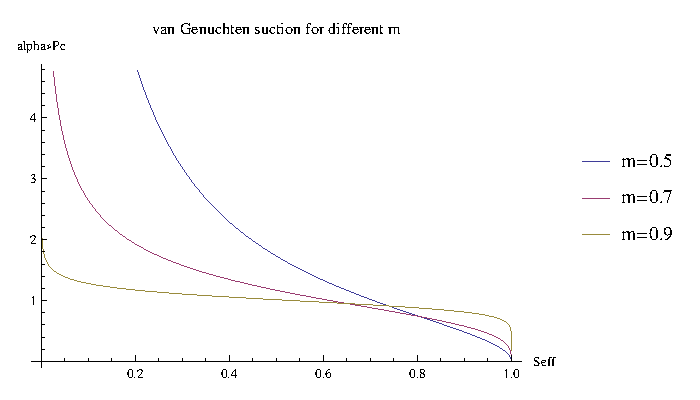
\includegraphics[width=10cm]{van_genuchten_pc.eps}
\caption{$\alpha P_{c}$ as a function of $S_{\mathrm{eff}}$ as given
  by van Genuchten's expression
  \hyperref[vg.cap.eqn]{Eqn~(\ref*{vg.cap.eqn})}.  Three values of $m$
  are shown: 0.5, 0.7 and 0.9 (the $m=0.5$ case has largest $P_{c}$
  around $S_{\mathrm{eff}}\sim 0$).}
\label{van_genuchten_pc.fig}
\end{figure}

\subsection{Broadbridge-White}

The Broadbridge-White\footnote{P Broadbridge, I White ``Constant rate rainfall
infiltration: A versatile nonlinear model, 1 Analytical solution''.
Water Resources Research 24 (1988) 145--154.} capillarity relationship
valid for small $K_{n}$ is
\begin{equation}
S_{\mathrm{eff}} = S_{n} + (S_{s} - S_{n}) \frac{c}{1 + L(x)} \ .
\end{equation}
where
\begin{equation}
x = (c - 1) e^{c - 1 - c P/\lambda} \ ,
\end{equation}
and $L(x)$ is the Lambert W-function that satisfies $L(z)e^{L(z)}=z$.
This is of limited use in real simulations, and is only used in the Porous
Flow module for comparison with the analytical solutions of
Broadbridge and White, and Warrick, Lomen and Islas\footnote{AW
  Warrick, DO Lomen and A Islas, ``An analytical solution to Richards'
  Equation for a Draining Soil Profile'', Water Resources Research 26
  (1990) 253--258.} for multi-phase infiltration and drainage
problems.

\subsection{Rogers-Stallybrass-Clements}

The Rogers-Stallybrass-Clements capillary relationship\footnote{C
  Rogers, MP Stallybrass and DL Clements ``On two phase filtration
  under gravity and with boundary infiltration: application of a
  Backlund transformation'' Nonlinear Analysis, Theory, Methods and
  Applications 7 (1983) 785--799} is
\begin{equation}
S_{\mathrm{eff}} = \frac{1}{\sqrt{1 + \exp((P_{c} - A)/B)}} \ ,
\label{eqn.rsc.seff}
\end{equation}
when the oil viscosity is exactly twice the water viscosity.  This is
of limited use in real simulations, and is only used in the Porous
Flow module for comparison with the analytical solutions offered by
the authors for multi-phase infiltration and drainage problems.


\section{Density}

For simple calculations with water, the fluid bulk modulus, $B$, may be
taken to be constant, so that the fluid density is
\begin{equation}
\rho = \rho_{0}e^{P/B} \ ,
\end{equation}
where $P$ is the fluid pressure.  It is common to use $\rho_{0} =
1000$\,kg.m$^{-3}$ and $B = 2$\,GPa.

\section{Tortuosity and diffusion coefficients}

The tortuosity may be constant, or it may follow the
Millington-Quirk\footnote{Millington and Quirk, Permeability of Porous
  Solids, Trans. Faraday Soc., 57, 1200- 1207, 1961} form
\begin{equation}
\tau_{\phase} = \phi^{1/3}S_{\phase}^{10/3}
\end{equation}
The molecular diffusion coefficients, $d_{\phase}^{\species}$, are
assumed to be constant.

\section{Effective fluid pressure}

The effective fluid pressure used in the definition of the fluid
effective stress \hyperref[eff.stress.eqn]{Eqn~(\ref*{eff.stress.eqn})} is
\begin{equation}
P = \sum_{\phase} S_{\phase}P_{\phase} \ .
\end{equation}

\section{Enthalpy and energy-density}

The specific enthalpy $h_{\phase}$, for a phase $\phase$, may be
defined using one of the high-precision equation of states (eg see
\hyperref[water.and.steam.sec]{Section~\ref*{water.and.steam.sec})},
or the relationship
\begin{equation}
h_{\phase} = \energydens_{\phase} + a P_{\phase}/\rho_{\phase} \ .
\end{equation}
It is usually appropriate to use $a=1$, however for comparison with
other codes it may be useful to use $a=0$.

The internal energy density $\energydens_{\phase}$ for a phase may be
defined using one of the high-precision equation of states, or the
relationship
\begin{equation}
\energydens_{\phase} = C_{v}T \ .
\end{equation}
may be used.


\section{Permeability}
\label{perm.sec}

The porous-material's insitu permeability tensor can be constant, or
it can take one of the following forms

\subsection{Exponential}

\begin{equation}
k_{ij} = k_{ij}^{0} e^{a\phi} \ ,
\end{equation}
where $\phi$ is the porosity, and $a$ is a user-defined constant.

\subsection{Kozeny-Carman}

Using the Kozeny-Carman relationship\footnote{Oelkers
1996: Reviews in Mineralogy v. 34, p. 131-192}
\begin{equation}
k_{ij} = k_{ij}^{0} \frac{\phi^{n}}{(1 - \phi)^{m}} \ .
\end{equation}
Here $n$ and $m$ are user-defined constants.

\subsection{\textcolor{red}{Permeability with a solid phase}}

\textcolor{red}{
A solid phase (from chemical precipitation, for instance) can be
included in the framework described herein simply by setting its
relative permeability to zero.  However, in this case, the absolute
permeability of the porous material should be
\begin{equation}
k = k^{\mathrm{without\ solid\ phase}}(1 - S_{\mathrm{s}})^{2} \ ,
\end{equation}
where $S_{\mathrm{s}}$ is the solid-phase saturation.
}

\section{Porosity}
\label{por.sec}

Porosity may be fixed at a constant value, or it may be a function of
the effective porepressure, the volumetric strain and/or the
temperature, as discussed below.

The evolution of the porosity\footnote{This is a generalisation of
  Eqn(18) in Y Chen, C Zhou and L Jing ``Modeling coupled THM
  processes of geological porous media with multiphase flow: Theory
  and vlidation against laboratory and field scale experiments''
  Computers and Geotechnics 36 (2009) 1308-1329} is governed by
\begin{equation}
\frac{\partial \phi}{\partial t} = (\alpha_{B} -
\phi)\frac{\partial}{\partial t}
\left(\epsilon^{\mathrm{total}}_{ii} - \alpha_{T} T\right) +
\frac{(1-\alpha_{B})(\alpha_{B}-\phi)}{K}\frac{\partial
  P_{f}}{\partial t} \ .
\label{eqn.phi.dog}
\end{equation}
Here $K$ is the bulk modulus of the drained porous skeleton: $1/K
= \delta_{ij}\delta_{kl}C_{ijkl}$.  This has solution
\begin{equation}
\phi = \alpha_{B} + (\phi_{0} - \alpha_{B})\times \exp \left( \frac{\alpha_{B}
  - 1}{K}P_{f} - \epsilon^{\mathrm{total}}_{ii} + \alpha_{T}T \right) \ ,
\label{poro.evolve.eqn}
\end{equation}
where $\phi_{0}$ is the porosity at zero porepressure, zero elastic
strain and zero temperature. Note this porosity can become negative.

The evolution of porosity is motivated further in the appendix
\hyperref[chap.evol.por]{Chapter~\ref*{chap.evol.por}}.

Without porepressure effects, the correct expression for porosity as a
function of volumetric strain and temperature is
\begin{equation}
\phi = 1 + (\phi_{0} - 1)\times \exp \left(- \epsilon^{\mathrm{total}}_{ii} + \alpha_{T}T \right) \ .
\end{equation}

\textcolor{red}{These expressions may be modified to include the
  effects of plasticity.}

\section{Relative permeability relationships}

The relative permeability of a phase is a function of its effective
saturation:
\begin{equation}
S_{\mathrm{eff}}(S) = \frac{S - S_{\mathrm{res}}^{\phase}}{1 -
  \sum_{\phase'}S_{\mathrm{res}}^{\phase'}}
\end{equation}
In this equation $S_{\mathrm{res}}^{\phase}$ is the residual
saturation for phase $\phase$.  If $S_{\mathrm{eff}} < 0$ then the
relative permeability is zero, while if $S_{\mathrm{eff}}>1$ then the
relative permeability is unity.  Otherwise, the relative permeability
is given by the expressions below.

\subsection{Constant}

\begin{equation}
k_{\mathrm{r}} = C \ .
\end{equation}
This is not recommended because there is nothing to discourage phase
disappearance, which manifests itself in poor convergence.  Usually
$k_{\mathrm{r}}(S) \rightarrow 0$ as $S\rightarrow 0$ is a much better
choice.

\subsection{Corey}

\begin{equation}
k_{\mathrm{r}} = S_{\mathrm{eff}}^{n} \ .
\end{equation}
where $n$ is a user-defined quantity.

\subsection{Broadbridge-White}

\begin{equation}
k_{\mathrm{r}} = K_{n} + \frac{K_{s} - K_{n}}{(c - 1)(c -
  S_{\mathrm{eff}})}S_{\mathrm{eff}}^{2} \ .
\end{equation}

\subsection{van Genuchten and cut van Genuchten}

\begin{equation}
k_{\mathrm{r}} = \sqrt{S_{\mathrm{eff}}} \left(1 - (1 -
S_{\mathrm{eff}}^{1/m})^{m} \right)^{2} \ .
\end{equation}
This has the numerical disadvantage that its derivative as
$S_{\mathrm{eff}}\rightarrow 1$ is crappy.  This means that
simulations where the saturation oscillates around
$S_{\mathrm{eff}}=1$ do not converge well.  Therefore, a ``cut''
version of the van-Genuchten expression is also offered, which is
almost definitely indistinguishable experimentally from the original
expression:
\begin{equation}
k_{\mathrm{r}} = \left\{
\begin{array}{ll}
\mbox{van Genuchten} & \mbox{ for } S_{\mathrm{eff}} < S_{c} \\
\mbox{cubic} & \mbox{ for } S_{\mathrm{eff}} \geq S_{c} \ .
\end{array}
\right.
\end{equation}
Here the cubic is chosen so that its value and derivative match the
van Genuchten expression at $S=S_{c}$, and so that it is unity at
$S_{\mathrm{eff}}=1$.

\subsection{FLAC}

\begin{equation}
k_{\mathrm{r}} = (n + 1)S_{\mathrm{eff}}^{n} - n S_{\mathrm{eff}}^{n +
  1} \ .
\end{equation}
This has the distinct advantage over the Corey formulation that its
derivative is continuous at $S_{\mathrm{eff}}=1$.



\section{Thermal conductivity}

Currently the Porous Flow module implements a
simple approach to the functional dependence of thermal conductivity
on the rock and fluid-phase conductivities.  A ``wet'' thermal
conductivity, $\lambda_{\mathrm{wet}}$, and a ``dry'' thermal
conductivity $\lambda_{\mathrm{dry}}$, are defined (both of which are
tensors), and
\begin{equation}
  \lambda = \lambda_{\mathrm{dry}} + S_{\mathrm{aqueous}}^{n}
  (\lambda_{\mathrm{wet}}-\lambda_{\mathrm{dry}})
\end{equation}
where $S_{\mathrm{aqueous}}$ is the aqueous phase saturation, and $n$
is a user-defined exponent.

\textcolor{blue}{The dependence of fluid thermal conductivity on temperature may be
handled within the fluid property modules (to accommodate
the kind of large changes that can occur when water flashes to
steam).}  \textcolor{red}{The solid thermal
conductivities also have a slight dependence on pressure, but it
sometimes difficult to obtain reliable data for these dependencies.}

\section{Viscosity}

Viscosity may be taken as constant, or the high-precision equations of
state may be used to define it.

\chapter{Implementation details and numerical issues}

\section{Independent (nonlinear) variables}

The Porous Flow module was designed from the ground up to be able to
employ variable switching, or persistent variables, instead of the
more common pressure-temperature-displacement set of variables.  Most
simulations in the test-suite use these common set of variables, but
it is up to the user to specify which variables are independent, and
which variables are dependent (usually the dependent variables will be
MOOSE AuxVariables).  A good choice of variables can lead to much
improved convergence.

\section{Lumping and upwinding}
\label{upwinding.and.lumping.sec}

The Porous Flow module employs fluid-mass and heat-energy lumping to
the nodes, as well as full upwinding of the advective flow terms.
This ensures far superior numerical convergence, especially in
situations where mass-fractions of phases are close to disappearing.

\subsection{Lumping}

Consider here just the fluid-flow equation, as the heat-energy
equation is analogous.  The time-derivative term in
\hyperref[mass.cons.sp.eqn]{Eqn~(\ref*{mass.cons.sp.eqn})} is discretised as
\begin{equation}
\psi \frac{M^{\species} - M^{\species}_{\mathrm{old}}}{\d t} \ .
\label{lump.begin.eqn}
\end{equation}
Here $\psi$ is the test function that we are integrating against.  An
alternative discretisation would be $\psi\phi(S\rho)'\dot{P}$ (in the
single-phase situation), but Eqn~(\ref{lump.begin.eqn}) conserves mass
more effectively than other alternatives.

In the standard finite-element scheme, $M^{\species}$ and its
individual parts (porosity, saturation, etc) are evaluated at each
quadrature point.  However, in PorousFlow, everything in the time
derivative is evaluated at the nodes.  Specifically, $M^{\species}$ at
a node depends only on the independent variables at that node.  It has
been shown in many papers that this lumping is advantageous for mass
conservation and reduces spurious oscillations of the pressure around
sharp fronts\footnote{MA Celia, ET Bouloutas and RL Zabra ``A general
  mass-conservative numerical solution for the unsaturated flow
  equation''  Water Resources Research 26 (1990) 1483--1496.}

The cause of oscillations around sharp fronts, and how mass lumping
removes the oscillations, can be illustrated through a simple example.

\begin{figure}[htb]
\centering
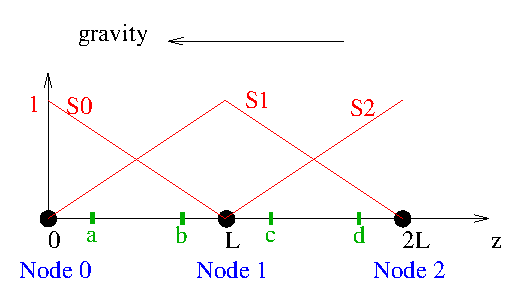
\includegraphics[width=9cm]{eg_richards_supg.eps}
\caption{Two elements of length $L$.  Linear Lagrange shape/test
  functions for each node are shown in red ($S_{0}$ for node 0,
  $S_{1}$ for node 1, and $S_{2}$ for node 2).  Gravity acts in the
  direction $-z$.  Gauss points are shown in green.}
\label{eg_richards_supg.fig}
\end{figure}

Consider the situation in
\hyperref[eg_richards_supg.fig]{Figure~\ref*{eg_richards_supg.fig}},
and suppose that Node 2 has high potential, and that nodes 0 and 1 are
at residual saturation where the relative permeability is zero.  Then
fluid will flow from node 2 to node 1 (and then to node 0 in the next
time step).  For simplicity, imagine that the fluid mass, $M$, is a linear
function of the potential.  Then, up to constants, the discretised
mass-conservation equation without mass lumping reads
\begin{equation}
\left(
\begin{array}{ccc}
2 & 1 & 0 \\
1 & 4 & 1 \\
0 & 1 & 2
\end{array}
\right)
\left(
\begin{array}{c}
\dot{M}_{0} \\
\dot{M}_{1} \\
\dot{M}_{2}
\end{array}
\right)
=
\left(
\begin{array}{c}
0 \\
1 \\
-1
\end{array}
\right)
\end{equation}
The matrix on the LHS comes from performing the numerical integration
of $M$ over the two elements.  Note that it is not diagonal
because the integration over an element depends on the mass at
both of its two nodes.  The RHS encodes that no fluid is flowing
between nodes 0 and 1, but fluid is flowing from node 2 to node 1.

The important point is the solution of these sets of equations is
\begin{equation}
\dot{M}_{0} < 0 \ .
\end{equation}
This means the finite element solution of the mass-conservation
equation will be oscillatory around fronts.

However, with mass lumping, the matrix in the above
equation becomes diagonal, and the solution is $\dot{M}_{0} =
0$.  Explicitly, the contribution to the residual at node $a$ is
\begin{equation}
\sum_{\mathrm{qp}}\psi_{a}^{\mathrm{qp}} \frac{M_{a}^{\species} -
  M^{\species}_{a,\ \mathrm{old}}}{\d t} \ .
\end{equation}
where $M$ is evaluated at node $a$ using the independent (Nonlinear)
variables evaluated at that node, and qp are the quadpoints.

There is one small complication.  Porosity may be dependent on
volumetric strain, which is dependent on the gradients of the
displacement variables, which are evaluated at the quadpoints, not the
nodes.  In this case, the porosity at node $a$ is assumed to be
dependent on the volumetric strain evaluated at the closest quadpoint
to the node.

\subsection{Upwinding}

Upwinding is necessary\footnote{Eg, see PS Huyakorn and GF Pinder ``A
  new finite element technique for the solution of two-phase flow
  through porous media'' Advances in Water Resources 1 (1978)
  285--298.  See also V Dalen ``Simplified finite-element models for
  reservoir flow problems'' SPEJ (Oct 1979) 333--343.  See also R
  Helmig and R Huber ``Comparison of Galerkin-type discretization
  techniques for two-phase flow in heterogeneous porous media''
  Advances in Water Resources 21 (1998) 697--711.} in scenarios with
nonlinear advection, such as the physics modelled by PorousFlow.  For
multi-phase situations many upwinding schemes can lead to disaster as
the algorithm attempts to withdraw fluid from a node where there is no
fluid.  I believe that for situations where one phase disappears, or
almost disappears, full upwinding is advisable, and hence PorousFlow
always employs full upwinding.  It has the numerical disadvantage that
it is not smooth (in contrast to the SUPG upwinding scheme\footnote{AN
  Brooks and TJR Hughes ``Streamline upwind/Petrov-Galerkin
  formulations for convection dominated flows with particular emphasis
  on the incompressible Navier-Stokes equations'' Computer Methods in
  Aplied Mechanics and Engineering 32 (1982) 199--259.  TJR Hughes and
  M Mallet ``A new finite element formulation for computational fluid
  dynamics: III. The generalized streamline operator for
  multidimensional advective-diffusive systems'' Computer Methods in
  Applied Mechanics and Engineering 58 (1986) 305--328.  TJR Hughes, M
  Mallet and A Mizukami ``A new finite element formulation for
  computational fluid dynamics: II. Beyond SUPG'' Computer Methods in
  Applied Mechanics and Engineering 54 (1986) 341--355}, for
instance), so that close to steady-state where the fluxes are zero,
the upwind direction can oscillate, leading to nonconvergence, however
this is dealt with by placing a cutoff on the upwinding in PorousFlow.
The remainder of this section describes full upwinding for the
single-phase unsaturated situation.  The multi-phase, multi-component
scenario, and the advective term in the heat-flow equation are
analogous.

The weak form of the Darcy flux of
\hyperref[darc.eqn]{Eqn~(\ref*{darc.eqn})} for a single element is
\begin{equation}
R_{a} = \int_{\mathrm{element}} \nabla_{i}\psi_{a}
\frac{\rho k_{ij}\,k_{\mathrm{r}}}{\mu}(\nabla_{j}P - \rho
g_{j})  \ .
\end{equation}
Here $\psi_{a}$ is the test function that we are integrating against,
and $R_{a}$ is the contribution to the residual for this test
function.  Define
\begin{equation}
m = \frac{\rho k_{\mathrm{r}}}{\mu} \ ,
\end{equation}
which is traditionally called the mobility.

Upwinding is all a matter of choosing where in the element to evaluate
$m$ in the above integral.  The sophisticated SUPG approach was
designed to weight $m$ on the upstream side of the element.  Consider
for a moment taking $m$ outside the integral:
\begin{equation}
\tilde{R}_{a} = m\int_{\mathrm{element}} \nabla_{i}\psi_{a}
\kappa_{ij}(\nabla_{j}P - \rho
g_{j}) = m I_{a} \ .
\end{equation}
$\tilde{R}$ is not exactly $R$, but note:
\begin{itemize}
\item the original $R_{a}$ is the mass flux flowing out of node $a$;
\item so $I_{a}$ is thereby intepreted as a measure of fluid flow out of
  node $a$.
\end{itemize}
This leads to the following definition of upwinding:
\begin{equation}
R_{a} \equiv m_{a}I_{a} \ \ \ \mbox{if}\ \ \ I_{a}\geq 0 \ .
\end{equation}
The nodes for which $I_{a}\geq 0$ are called ``upwind nodes'', since
fluid is flowing from them to the ``downwind nodes''.  I think this
approach was first introduced by Dalen\footnote{V Dalen ``Simplified
  finite-element models for reservoir flow problems'' SPEJ (Oct 1979)
  333--343} in 1979.

The residual at the downwind nodes is determined by conserving mass.
Specifically, let
\begin{equation}
I_{\mathrm{up}} = \sum_{I_{a}\geq 0}I_{a} \ \ \ \mbox{and}\ \ \
I_{\mathrm{down}} = -\sum_{I_{a}<0} I_{a} \ .
\end{equation}
Then
\begin{equation}
R_{a} = I_{a}\frac{I_{\mathrm{up}}}{I_{\mathrm{down}}}
\ \ \ \mbox{for}\ \ \ I_{a}<0 \ .
\end{equation}
Then $\sum_{a} R_{a} = 0$ as required by mass conservation within the
element (which originates from $\sum_{a} \psi_{a} = 1$).

The fully-upwind method is extremely
advantageous to use if fluid saturations ever approach residual
saturation (where $\kappa_{\mathrm{rel}}=0$) or zero density, for then
the mobility is zero and it becomes impossible to withdraw fluid from
such a node (in practice this may still happen due to precision loss
or other related nasty artifacts that I will not describe here).

Prescribed sinks, either from the boundary or from internal objects
such as wellbores, are also fully-upwinded in PorousFlow since they
also potentially suffer from phase-disappearence problems.

\section{Preconditioners and linear solvers}

MOOSE allows users to utilise the full power of the PETSc
preconditioners and linear solvers.  The following choices have been
found to be effective for various types of PorousFlow simulations.
\begin{itemize}
\item {\tt pc\_type = bjacobi, ksp\_type = bcgs}.
\item {\tt pc\_type = bjacobi, ksp\_type = gmres}.
\item {\tt pc\_type = asm, pc\_asm\_overlap = 2, sub\_pc\_type = lu,
  sub\_pc\_factor\_shift\_type = NONZERO, 
  ksp\_type = gmres}.
\item {\tt pc\_type = asm, pc\_asm\_overlap = 2, sub\_pc\_type = lu,
  sub\_pc\_factor\_shift\_type = NONZERO, 
  ksp\_type = gmres} along with the following options {\tt
  -ksp\_diagonal\_scale -ksp\_diagonal\_scale\_fix
  -ksp\_gmres\_modifiedgramschmidt}.
\end{itemize}


%%%%%%%%%%%%%%%%%%%%%%%%%%%%%%%%%%%%%%%%%%%%%%%%%%%%%%%

\appendix

\chapter{The continuity equation}

The derivation of the continuity equation is fundamental to the fluid
and heat flow DEs, and is
included in this section.  The notation in this appendix is different
from that in the main report.

\section{Eulerian coordinates}

Introduce the notion of the ``spatial coordinate frame''.  It is the
coordinate frame of a stationary observer who is looking at the
deforming porous solid from the outside.  Denote its coordinates by
${\mathbf x}$, and the derivatives with respect those coordinates by
$\nabla$.

Let $\Omega$ be a volume that is attached to particles of the
porous-solid skeleton.  As the porous solid deforms, so too will
$\Omega$.  Denote the velocity of the porous solid is ${\mathbf
  v}_{s}$, measured in the spatial coordinate frame: ${\mathbf v}_{s}
= {\mathbf v}_{s}(x, t)$.  Then the change of a small volume element
$\d\Omega$ is computed by calculating the Jacobian, and it is
\begin{equation}
\frac{\d}{\d t} (\d\Omega) = \nabla\cdot{\mathbf v}_{s} \d\Omega \ .
\end{equation}
Remember the derivative $\nabla$ is differentiating with respect to
the coordinates of the spatial coordinate frame.  This formula is easy
to motivate because $\nabla\cdot{\mathbf v}_{s} = \dot{\epsilon}_{ii}$
which is the time derivative of the volumetric strain.

Let $M$ represent a quantity that is attached to the porous-solid
skeleton, for instance the mass density of the solid.  Express $M$ in
the spatial coordinate frame: $M=M(x, t)$.  As the porous
solid deforms
\begin{equation}
\frac{\d}{\d t}M = \frac{\partial}{\partial t}M + {\mathbf v}_{s}\cdot
\nabla M \ .
\end{equation}
The second term is easy to motivate if you consider a constant
velocity with the spatially-dependent but temporally-constant $M$.

The continuity equation is
\begin{equation}
\frac{\d}{\d t}\int_{\Omega}M \d\Omega + \int_{\partial
  \Omega}{\mathbf F}\cdot{\mathbf n}\,\d A = 0 \ ,
\end{equation}
where ${\mathbf F}$ is the flux of $M$ out of $\Omega$, $n$ is the
outward unit normal, and $\d A$ is the area element on
$\partial\Omega$ (which is the surface of $\Omega$).  Using the above
expressions, and the divergence theorem, the continuity equation reads
\begin{equation}
\int_{\Omega} \left( \frac{\partial}{\partial t}M + \nabla\cdot(M{\mathbf
  v}_{s}) + \nabla\cdot{\mathbf F}  \right)\d\Omega = 0 \ .
\label{equation.continuity.eul}
\end{equation}
Specialising $M$ and ${\mathbf F}$ to fluids and heat gives the
equations mentioned in the main text.


\section{Lagrangian coordinates}

Introduce the notion of the ``material coordinate frame''.  It is the
coordinate frame of an observer who is fixed to a certain point in the
porous solid (eg, a particular finite-element node).  Denote the
coordinates in this frame by $X$.  This is the
frame used throughout this report.  Fluid properties (pressures, mass
fractions), the temperature, etc, are all stored at the finite-element
nodes or the quadpoints, and move with the mesh.  At the very least,
an Eulerian description would be inconvenient when visualising with
paraview.

Introduce the material derivative $\mathrm{D}/\mathrm{D} t$.  If $M$
is any property that is expressed in terms of the ``spatial coordinate
frame'' (Eulerian coordinates): $M=\tilde{M}(x,t)$, then the material
derivative is
\begin{equation}
\frac{\mathrm{D}}{\mathrm{D} t}\tilde{M}(x, t) = \frac{\partial
}{\partial t}\tilde{M}(x, t) + {\mathbf{v}}_{s}\cdot \nabla
\tilde{M}(x, t)\ .
\end{equation}
The continuity
\hyperref[equation.continuity.eul]{Eqn~(\ref*{equation.continuity.eul})}
can be re-written as
\begin{equation}
0 = \frac{\mathrm{D}}{\mathrm{D} t}M + M\nabla\cdot {\mathrm{v}}_{s}
\ .
\end{equation}
However, if $M$ is expressed in terms of the Lagrangian coordinates:
\begin{equation}
M = M(X, t) \ ,
\end{equation}
(generally $M(X, t)$ will have a different functional form than
$\tilde{M}(x,t)$, thus the tilde to emphasise the difference)
then the material derivative is expressed by
\begin{equation}
\frac{\mathrm{D}}{\mathrm{D} t}M(X, t) = \frac{\partial}{\partial
  t}M(X, t) \ ,
\end{equation}
but the continuity equation has the identical form:
\begin{equation}
0 = \frac{\mathrm{D}}{\mathrm{D} t}M + M\nabla\cdot {\mathrm{v}}_{s}
\ .
\end{equation}


\chapter{Benchmark studies to perform}


\section{Use case: Two-component, two-phase, nonisothermal}

This solution will benchmark the two-phase immiscible flow and thermal equations in of the code against the semi-analytical solutions in LaForce et al (AWR, 73 (2014a) $227 - 241$). (Note: These will have to be written because they are copy/pasted from manuscript)

The analytical solutions assume that pressure changes in the reservoir are small, so that fluid volume, density, and viscosity are all constant. Fluids and the solid are treated as incompressible.  It is also assumed that changes in temperature do not impact any of the solid or fluid properties.  With these assumptions the thermal and saturation equations become

\begin{eqnarray}
&&\left[ S_1  + \beta \right]\frac{\partial T_{D1}}{\partial t_D} +
\left[  f_1  + \alpha\right] \frac{\partial {D1}}{\partial r_D} = k_{Tt}\gamma_j \frac{\partial^2 {D1}}{\partial z_D^2} \label{eqn:generic_T}\\
&&\frac{\partial S_1}{\partial t_D } + \frac{\partial f_1}{\partial r_D } = 0 \label{eqn:generic_S}
\end{eqnarray}
\begin{eqnarray}
&&\alpha = \frac{\rho_2  C_2}{\left(\rho_1  C_1  - \rho_2  C_2 \right)} \label{eqn:alpha}\\
&&\beta = \frac{\rho_2  C_2  + \frac{ 1-\phi_r }{\phi_r}\rho_s C_s }{\left(\rho_1  C_1  - \rho_2  C_2 \right)} \label{eqn:beta}
\end{eqnarray}

\noindent where $S_1$ is the saturation of the water phase, $f_1$ is
the fractional flow of the water (resident) phase, $T_{D1}$ is
temperature and $r_D$ is radial distance.  The $C_j$ are the
mass-based heat capacity of fluid 1, 2, or the formation rock.  The
parameters $\alpha$ and $\beta$ in
\hyperref[eqn:alpha]{Eqns~\ref*{eqn:alpha}}---\hyperref[eqn:beta]{(\ref*{eqn:beta})}
are constant throughout the displacement.  Dimensionless variables are
defined in LaForce et al (2014a).

%For one dimensional radial flow the dimensionless variables and linear heat loss coefficient, $\gamma_j=\gamma_R$, are defined as:
%
%\begin{eqnarray}
%z_D &=& \frac{z}{h}  \label{eqn:zD}\\
%T_{D1} &=& \frac{T-T_i}{T_{w}-T_i}  \label{eqn:TD}\\
%r_D &=& \frac{r^2}{L^2}\label{eqn:r_D} \\
%t_D &=& \frac{q t }{\pi \phi_r L^2 h }\label{eqn:t_D_r} \\
%\gamma_R &=& \frac{L^2 \pi }{q\left(\rho_1  C_1  - \rho_2  C_2 \right)}\label{eqn:gamma_R}
%\end{eqnarray}
%
%\noindent where $L$ is length of the porous medium, $h$ is the
%vertical thickness of the porous medium, $q$ is volumetric injection
%rate, $T_i$ is initial reservoir temperature and $T_w$ is injection
%temperature at the well, which may be larger or smaller than the
%reservoir temperature.

The relative permeability of the phases are from one of the TOUGH2 models


\begin{eqnarray}
k_{r1} &=& \hat{S}^4 \nonumber\\
k_{r2} &=& \left(1-\hat{S}\right)^2 \left(1-\hat{S}^2\right)\\
\hat{S} &=& \frac{S_1-S_{1r}}{1-S_{1r}-S_{2r}}\nonumber
\end{eqnarray}

In the analytical model, heat loss from the reservoir to the over/under burden is handled via a heat sink term that approximates the diffusive process.

\begin{equation}
k_{Tt}\frac{\partial^2 T_D}{\partial z^2} \to -U T_D.
\end{equation}

\noindent Note: It may be useful to solve these equations with $U=0$ initially.


%\noindent where

%\begin{eqnarray}
%&&U(t_D) = \sqrt{\frac{q K_{a}(\rho C)_{a}}{t_D \pi \phi_r L^2 h }}. \label{eqn:U_L}
%\end{eqnarray}
%
%\noindent $(\rho C)_{a} = (1-\phi_a) \rho_a C_a +  \phi_a \rho_1 C_1
%$.  The $C_j$ are the mass-based heat capacity of fluid 1, 2, or the
%adjacent formation rock, and $K_a$ is the saturated thermal
%conductivity of the adjacent formations.

In this formulation the thermal properties of the reservoir and the
adjacent formations may be different, but the over- and under-burden
must have the same thermal properties for vertical symmetry.  It will
be interesting to test the simulator on the full
\hyperref[eqn:generic_T]{Eqn~(\ref*{eqn:generic_T})} with vertical
heat diffusion vs a simulated solution with the heat sink.


\section{Two-component, two-phase, nonisothermal, forward coupled stress}

This solution will benchmark the code against the semi-analytical solutions in LaForce et al (AWR, 73 (2014) $242 - 253$), which takes the saturation and temperature solution from above and also calculates pressure and stress in the reservoir.  The semi-analytical solutions are strictly forward-coupled, so that pressure does not impact the saturation or temperature profiles, and stress has no impact on pressure, saturation or temperature. In that work, pressure and stress are calculated at a given snapshot in time, $t_D^*$. This gives pressure and stress equations with no time dependence:

\begin{eqnarray}
&&\frac{\partial P}{\partial r_D} = \frac{q}{4\pi h k r_D}
  \frac{1}{M}\label{eqn:P_again}
\end{eqnarray}

\noindent where $M$ is the mobility of the overall fluid composition
at $r_D$.

The displacement $u$, of the porous medium at a fixed time is given by
{\bf Note: Notation may not be consistent with the above!!}:

\begin{eqnarray}
&&\frac{d}{d \xi}\left(\frac{1}{\xi}\frac{d}{d \xi}(\xi u_D)\right) = \frac{\partial T_{D2}}{\partial \xi}+
\frac{(1-2\nu)}{(1-\nu)}\frac{\partial P_D}{\partial \xi}\label{eqn:disp_u}
\end{eqnarray}

\noindent where $\xi = \frac{r}{r_w}$ for well radius $r_w$, and $\nu$ is the drained Poisson ratio.  All other dimensionless groups given in LaForce et al (2014b).

%\begin{eqnarray}
%P_D & = & \frac{(P- P_{o})(1-\nu)}{\alpha T_r E}\\
%T_{D2} & = & \begin{cases} T_{D1}, & \mbox{if } T_r \leq
%0\vspace{0.25cm} \label{eqn:TD2}\\
%-T_{D1}, &  \mbox{if } T_r > 0 \end{cases}\\
%u_D & = & \frac{u(1-\nu)}{\alpha T_r r_w (1+\nu)}\\
%\epsilon_{D,j} & = & \frac{\epsilon(1-\nu)}{\alpha T_r (1+\nu)}\\
%\sigma_{D,j} & = & \frac{(\sigma_j - \sigma_{hD})(1-\nu)}{\alpha T_r E}\\
%\xi & = & \frac{r}{r_w}
%\end{eqnarray}

%\noindent where $\nu$ is the drained Poisson ratio, $E$ is the
%drained Young's modulus of the rock, $\alpha$ is the Biot
%pore-pressure coefficient (coefficient of linear thermal expansion),
%$P_o$ is the original pore pressure in the reservoir and $r_w$ is the
%well radius.  $T_r = T_i-T_w$ is the relative temperature and the
%dimensionless temperature is re-defined so that the injection
%temperature is -1.0 when cold fluid is injected ($T_r>0$) and +1.0
%when hot fluid is injected ($T_r\leq 0$).  $\xi$ is a new
%dimensionless radial distance that is convenient for the
%stress/strain equations.  The length of the domain  $\xi_1=L/r_w$
%must be the same as the length of the temperature and pressure
%domain. Strain is denoted by $\epsilon_j$ and $\sigma_j$ is stress,
%where $j$ can denote either a radial ($j=r$) or tangential
%($j=\Theta$) variable.   Similarly $\epsilon_{D,j}$ and
%$\sigma_{D,j}$ denote dimensionless strain and stress, where $j$ can
%denote either the dimensionless radial ($j=\xi$) or tangential
%($j=\theta$) variable.   $\sigma_r^e=\sigma_r + P$ is the effective
%radial stress.

In these equations stresses are defined as positive if they are tensile and negative if they are compressive. The stress at the wall of the well will have equal magnitude as the fluid pressure, but opposite sign so that at the wellbore the effective radial stress is always zero.  These equations can be solved analytically on a finite reservoir domain for either zero stress or zero displacement outer boundary conditions.

%The boundary conditions at a given time $t^*$ for constant rate and temperature injection of a fluid into a well in a reservoir of length $\xi_1$ with an open boundary are:
%
%\begin{eqnarray}
%\frac{\partial P_D(1,t^*)}{\partial r} &=& \frac{-q \mu_{inj}}{2 \pi k h} \frac{(1-\nu)}{\alpha T_w E}\label{eqn:BCs}\\
%T_{D2}(1,t^*) &=& T_{D2,w}\nonumber\\
%\sigma_{D,\xi}(1,t^*) &=& - (P_{Dw}(t^*) + P_{o,D}) - \sigma_{hD}\nonumber\\
%P_D(\xi_1,t^*) &=& 0\nonumber\\
%T_D(\xi_1,t^*) &=& 0.\nonumber\\
%\nonumber
%\end{eqnarray}
%

\chapter{Evolution of porosity for an isothermal situation}
\label{chap.evol.por}

The evolution of porosity is fundamental to the coupling between flow
and solid mechanics.  Consider the isothermal situation with no
plasticity.

Denote the change of a quantity, q, by $\Delta
q$.  Recall that the porosity is defined by $\phi = V_{\mathrm{f}}/V$,
where $V$ is an arbitrary volume of the porous material, and
$V_{\mathrm{f}}$ is the porevolume within that volume.  Also, by
definition of the effective stress,
\begin{equation}
\Delta \epsilon_{ij} = C_{ijkl}(\Delta\sigma_{ij}^{\mathrm{tot}}  + \alpha_{B}
\delta_{ij}\Delta P_{\mathrm{f}})
\ .
\end{equation}
Taking the trace of this equation, and using $V^{-1}\Delta V = \Delta
\epsilon_{ii}$ yields
\begin{equation}
\frac{\Delta V}{V} = \delta_{ij}C_{ijkl}(\Delta\sigma_{ij}^{\mathrm{tot}}+
\alpha_{B} \delta_{ij}\Delta P_{\mathrm{f}})
\ .
\end{equation}
In most instances it is appropriate to write this equation as
\begin{equation}
\frac{\Delta V}{V} = -\frac{1}{K}(\mechpressure - \alpha_{B} \delta_{ij}\Delta P_{\mathrm{f}})
\ .
\label{eqn.fund.volstrain}
\end{equation}
where the total mechanical pressure is
\begin{equation}
\mechpressure = - \mbox{Tr}\sigma/3 \ .
\end{equation}
and $K$ is the so-called ``drained'' bulk modulus $K = \delta_{ij}C_{ijkl}\delta_{kl}$.
To find the evolution equation for porosity, a similar equation for
$\Delta V_{\mathrm{f}}/V_{\mathrm{f}}$ must be derived.

Assuming linearity
\begin{equation}
\frac{\Delta V_{\mathrm{f}}}{V_{\mathrm{f}}} = A_{ij}
(\Delta\sigma_{ij}^{\mathrm{tot}} + B \delta_{ij}\Delta
P_{\mathrm{f}}) \ .
\label{eqn.deltavf}
\end{equation}
The Betti-Maxwell reciprocal theorem yields $A_{ij}$ and $B$, as is
now shown.

The work increment is
\begin{equation}
\d W = -\mechpressure \d V + P_{\mathrm{f}} \d V_{\mathrm{f}} \ ,
\end{equation}
So during some deformation that takes $\mechpressure$ from
$\mechpressure^{i}$ to $\mechpressure^{f}$, and $P_{\mathrm{f}}$ from
$P_{\mathrm{f}}^{i}$ to $P_{\mathrm{f}}^{f}$, the total work is
\begin{eqnarray}
W & = & -\int \mechpressure\d V + \int P_{\mathrm{f}}\d V_{\mathrm{f}}
\ , \nonumber \\ & = &
\frac{V}{K}\int_{\mechpressure^{i}}^{\mechpressure^{f}}\mechpressure
\d \mechpressure -
\frac{V{\alpha_{B}}}{K}\int_{P_{\mathrm{f}}^{i}}^{P_{\mathrm{f}}^{f}}\mechpressure
\d P_{\mathrm{f}} +
V_{\mathrm{f}}A_{ii}\int_{\mechpressure^{i}}^{\mechpressure^{f}}P_{\mathrm{f}}
\d \mechpressure +
V_{\mathrm{f}}A_{ii}B\int_{P_{\mathrm{f}}^{i}}^{P_{\mathrm{f}}^{f}}
P_{\mathrm{f}} \d P_{\mathrm{f}} \ .
\end{eqnarray}
Now consider two experiments:
\begin{enumerate}
\item First take $\mechpressure$ from $0$ to $\mechpressure$ with
  $P_{\mathrm{f}}$ fixed at $0$.   Then,
  leaving $\mechpressure$ fixed, take $P_{\mathrm{f}}$ from $0$ to
  $P_{\mathrm{f}}$.  The first takes work $V\mechpressure^2/(2K)$,
  while the second takes work $-{\alpha_{B}} V\mechpressure P_{\mathrm{f}}/K +
  V_{\mathrm{f}}A_{ii}B P_{\mathrm{f}}^{2}/2$.
\item First take $P_{\mathrm{f}}$ from $0$ to $P_{\mathrm{f}}$ with
  $\mechpressure$ fixed at $0$.   Then,
  leaving $P_{\mathrm{f}}$ fixed, take $\mechpressure$ from $0$ to
  $\mechpressure$.  The first takes work
  $V_{\mathrm{f}}A_{ii}B P_{\mathrm{f}}^{2}/2$, and the
  second takes work  $V\mechpressure^{2}/(2K) +
  V_{\mathrm{f}}\mechpressure A_{ii}P_{\mathrm{f}}$.
\end{enumerate}
The two experiments must give the same work done (this is called the
Betti-Maxwell reciprocal theorem), which yields
\begin{equation}
A_{ij} = \alpha_{B} C_{ijkl}\delta_{kl}/\phi \ .
\label{tildek.eqn}
\end{equation}

Now to identify $B$.  Consider a so-called
``ideal porous material'', which is characterised by a fully-connected
pore space and a homogeneous and isotropic matrix material.  In this
case, applying a uniform porepressure, $P_{f}$, and an equal
mechanical pressure, $\mechpressure=P_{f}$, the solid material
will experience a uniform pressure throughout its skeleton.   This
means it will deform uniformly without any shape change, and
\begin{equation}
\frac{\Delta V_{\mathrm{f}}}{V_{\mathrm{f}}} = \frac{\Delta V}{V} \ .
\end{equation}
Substituting this equation, this specific pressure condition, and
\hyperref[tildek.eqn]{Eqn~(\ref*{tildek.eqn})} into
\hyperref[eqn.fund.volstrain]{Eqns~(\ref*{eqn.fund.volstrain})}
and~\hyperref[eqn.deltavf]{(\ref*{eqn.deltavf})}, yields
\begin{equation}
B = 1 + \phi - \phi/{\alpha_{B}} \ .
\end{equation}

Now that $A_{ij}$ and $B$ have been identified, they may be
substituted into \hyperref[eqn.deltavf]{Eqn~(\ref*{eqn.deltavf})}.  Rearranging yields
\begin{equation}
\frac{\Delta V_{\mathrm{f}}}{V_{\mathrm{f}}} =
\frac{\alpha_{B}}{\phi}\delta_{ij}C_{ijkl} \left[ \Delta
\sigma_{kl}^{\mathrm{tot}} + \alpha_{B} \delta_{kl} \Delta P_{\mathrm{f}}
\right] +
\frac{\delta_{ij}\delta_{kl}C_{ijkl}}{\phi}(1-\alpha_{B})(\alpha_{B}-\phi)\Delta
P_{f}
\end{equation}
Using the expression for $\Delta V/V$ yields
\begin{equation}
\Delta V_{\mathrm{f}} = V\alpha_{B}\Delta\epsilon_{ii} +
V\delta_{ij}\delta_{kl}C_{ijkl}(1-\alpha_{B})(\alpha_{B}-\phi)\Delta P_{f}
\end{equation}
Now $\Delta\phi = V^{-1}\Delta V_{\mathrm{f}} -
V_{\mathrm{f}}V^{-2}\Delta V$, so using the definition of $K$
yields
\begin{equation}
\frac{\partial \phi}{\partial t} = (\alpha_{B} - \phi)\frac{\partial
  \epsilon_{ii}}{\partial t} + \frac{(1-\alpha_{B})(\alpha_{B} -
  \phi)}{K}\frac{\partial P_{\mathrm{f}}}{\partial t} \ ,
\end{equation}
as written in \hyperref[eqn.phi.dog]{Eqn~(\ref*{eqn.phi.dog})}.

\end{document}

